% This file is included by MIT-Thesis.tex as an appendix chapter.
% Adapted from the MindControl paper-tex supplement.tex. Section/equation
% labels prefixed with interareal-control- to disambiguate from other
% chapters' appendices; cross-references to "Methods Eq.~N" in the source
% supplement have been rewritten to point at the chapter equations defined
% in sections/interareal-control.tex.

\chapter{Methods: Disruption of interareal control during propofol anesthesia}
\label{chap:interareal-control-appendix}

\section{Supplementary results}\label{supp:interareal-control-results}

\subsection{Linearity of the learned dynamics and linear baseline analysis}\label{supp:interareal-control-linearity}

A natural question raised by the conditional JacobianODE model is whether the dynamics it learns from the propofol cohort are genuinely nonlinear, or whether a strictly linear time-invariant (LTI) description of the same data would suffice. We address this question along two complementary axes (Figure~\ref{fig:interareal-control-linearity}). The first axis (panels~A,B) interrogates the JacobianODE model itself: how strongly does the learned Jacobian vary along the trajectory, and how does that variation trade off against predictive accuracy? The second axis (panels~C,D) replaces the learned Jacobian altogether with a linear delay-embedded model and asks whether the same anesthesia-related Gramian reorganization survives this substitution.

\begin{figure}[tp]
\centering
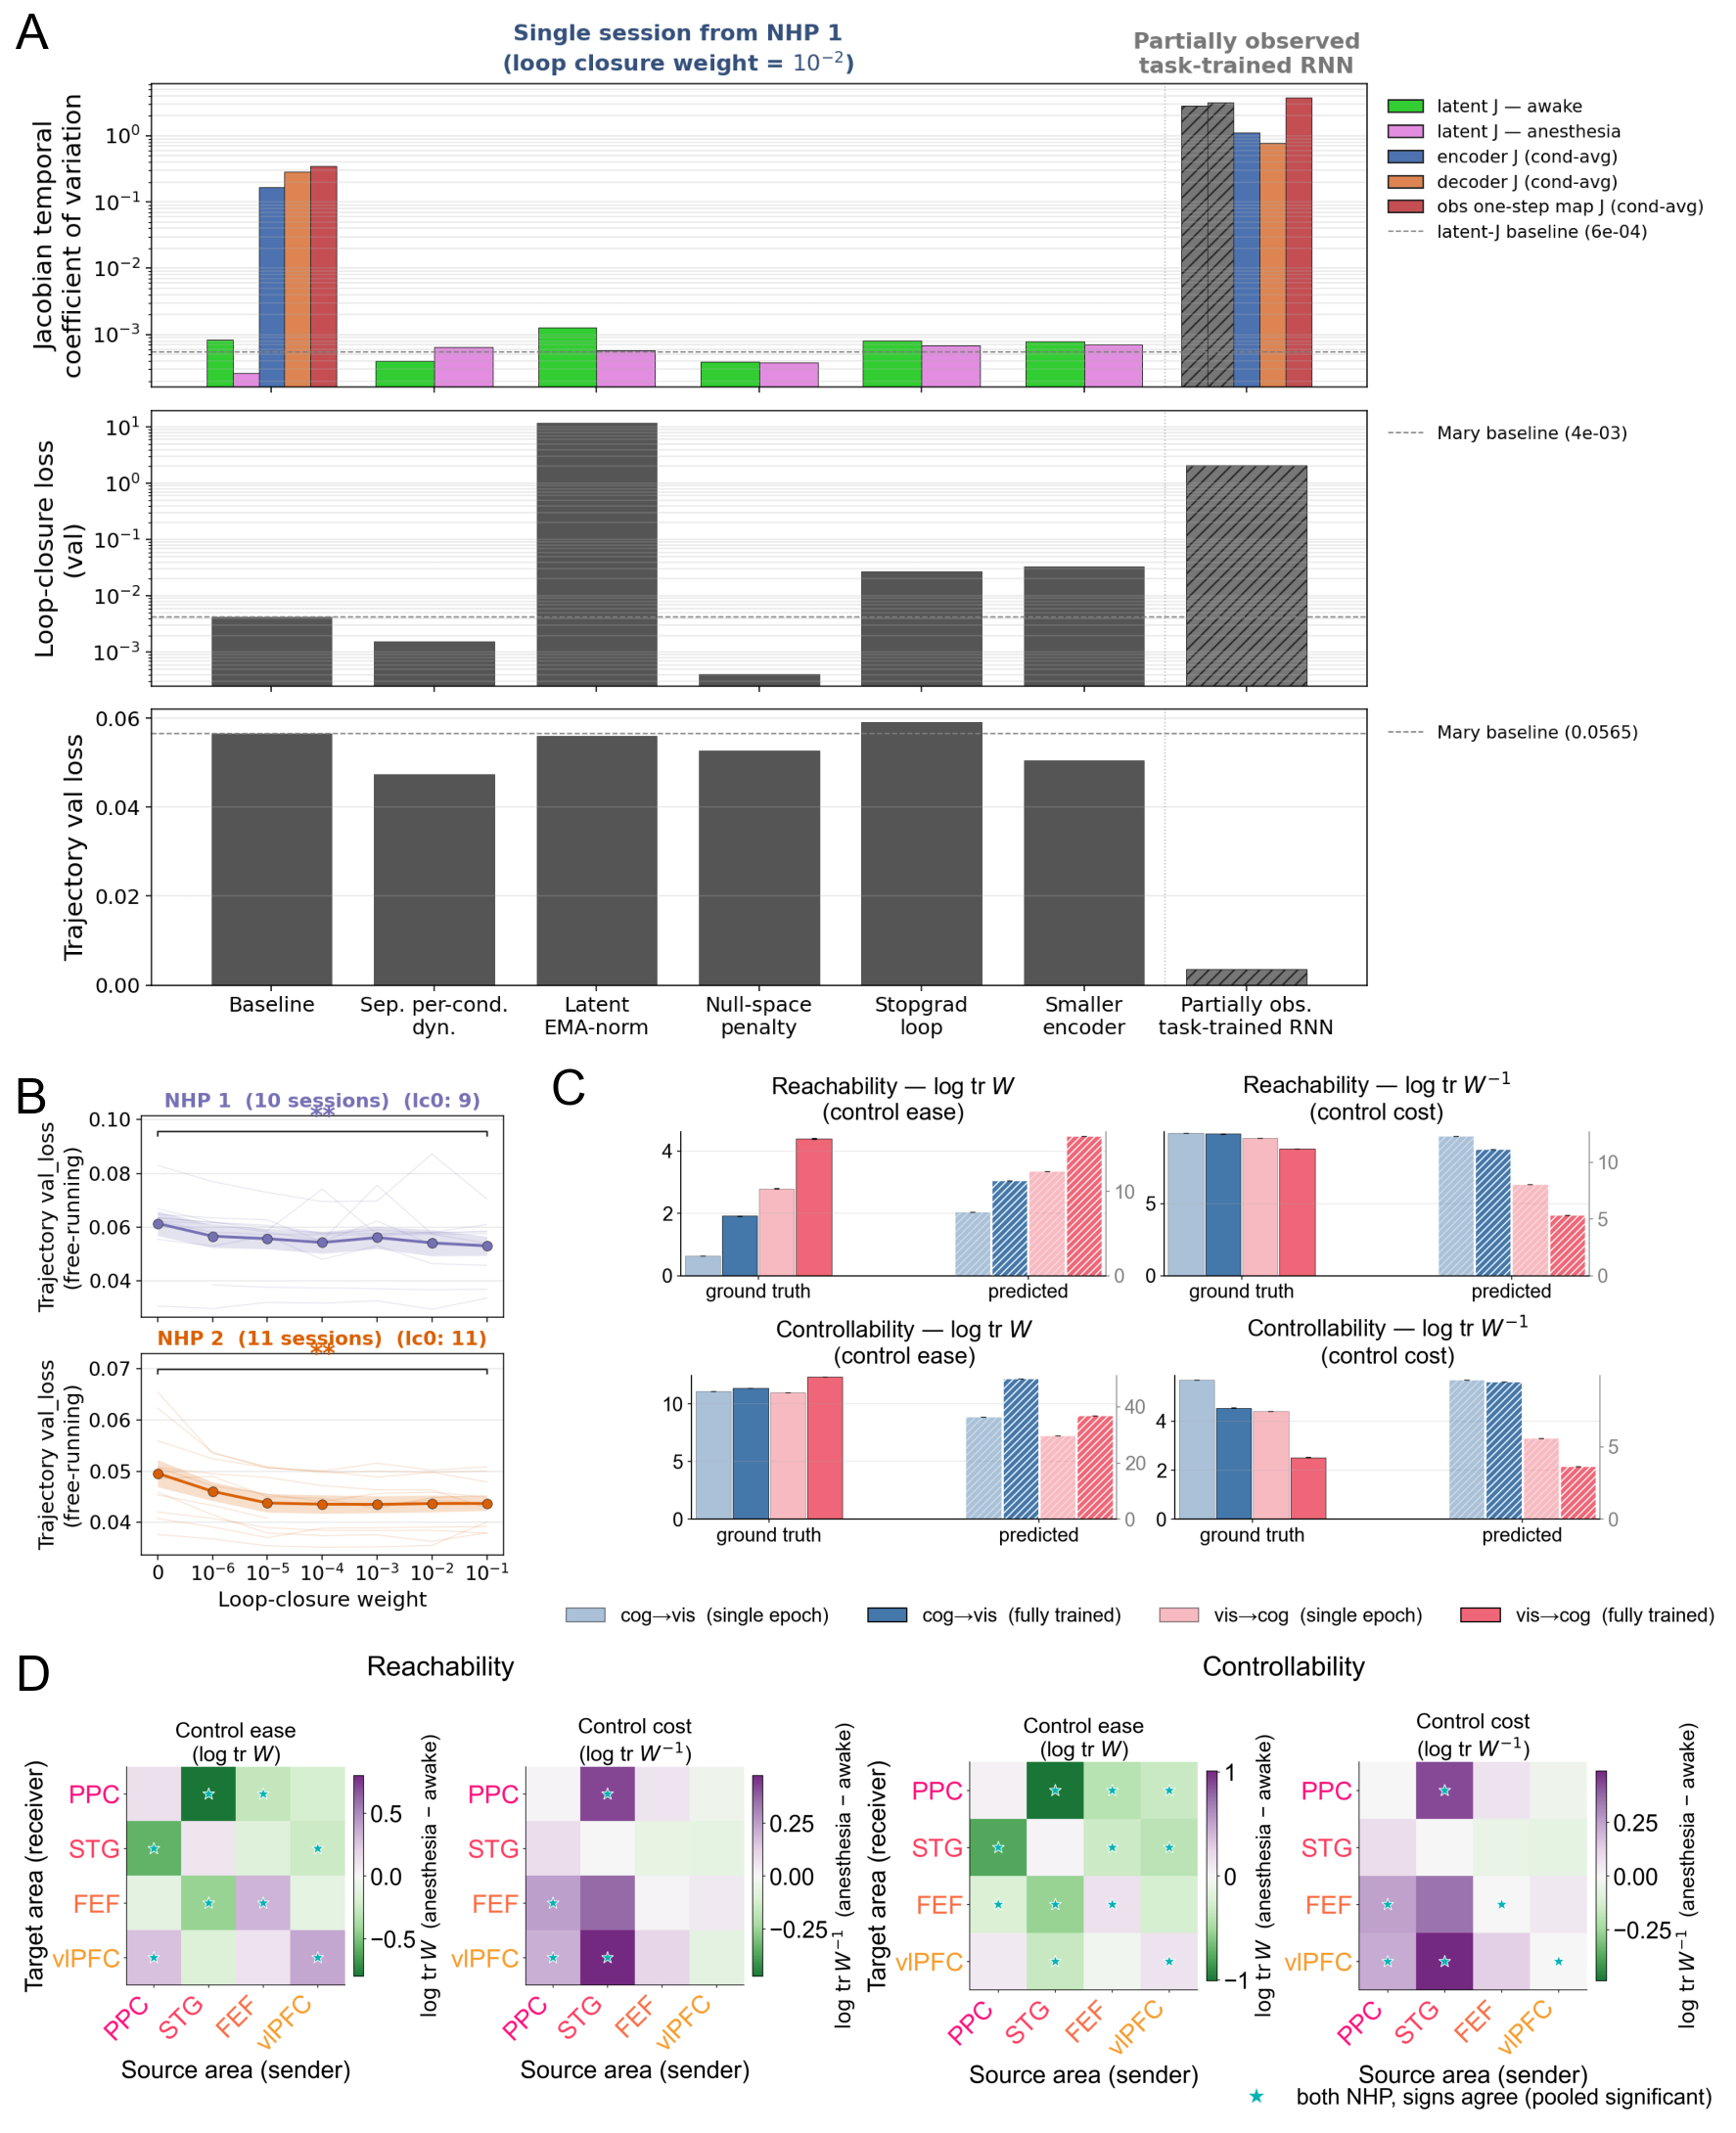
\includegraphics[width=\linewidth,height=0.74\textheight,keepaspectratio]{figures/interareal-control/fig_methodology_composite.png}
\caption[Linearity diagnostics and linear delay-embedded baseline]{\textbf{Linearity diagnostics and linear delay-embedded baseline.} \textbf{(A)}~Six anti-LTI interventions on a single session from NHP 1 (using loop-closure weight $10^{-2}$), with a partially observed task-trained RNN as nonlinear reference. (A, top) Per-condition latent Jacobian temporal coefficient of variation (CV), used as a measure of nonlinearity. The condition-averaged encoder ($\mathbf{J}_{\vb{\Psi}}$), decoder ($\mathbf{J}_{\vb{\Psi}^{-1}}$), and round-trip Jacobian CV area overlaid for the baseline and the RNN reference. (A, middle) Validation loop-closure loss. (A, bottom) Free-running trajectory validation loss. The NHP 1 variants cluster near the baseline on all three latent-Jacobian diagnostics. The encoder/decoder Jacobians, by contrast, are two to three orders of magnitude more state-dependent (Eq.~\ref{eq:supp-interareal-control-obs-jac-chain}), and the reference shows the genuinely nonlinear regime the architecture is capable of. \textbf{(B)}~Best free-running trajectory validation loss vs.\ loop-closure weight $\lambda_{\mathrm{loop}}$, per NHP, across the cohort's chosen-cell sweep grid (per-session lines + mean $\pm$ SEM). There is a monotone-non-decreasing trend in both NHPs, indicating improved fits with models that obey loop closure laws.. \textbf{(C)}~Per-area linear delay-embedded baseline (Eqs.~\ref{eq:supp-interareal-control-lin-svd}--\ref{eq:supp-interareal-control-lin-dmd}) applied to the partially observed task-trained RNN. Reachability and controllability gramian and inverse gramian log traces ($\log\mathrm{tr}\,\mathbf{W}$ and $\log\mathrm{tr}\,\mathbf{W}^{-1}$) for the visual~$\to$~cognitive and cognitive~$\to$~visual blocks at single-epoch and fully-trained checkpoints. Ground truth (left of each pair) vs.\ linear baseline (right). \textbf{(D)}~The same linear baseline on the propofol cohort, with the four sign-agree pooled-Wilcoxon $4\!\times\!4$ Gramian $\Delta$-heatmaps that mirror Figure~\ref{fig:interareal-control-neural-control}A,B of the chapter. The qualitative reorganization is preserved, with smaller effect sizes and more variability.}
\label{fig:interareal-control-linearity}
\end{figure}

\paragraph{The learned Jacobian is approximately linear despite targeted anti-LTI interventions.}
For one representative session of the propofol cohort (NHP~1, loop-closure weight $\lambda_{\mathrm{loop}}=10^{-2}$) we compared the production baseline against six anti-LTI variants designed to push the Jacobian off the constant-matrix solution: separate per-condition dynamics, a per-batch latent exponential moving average normalization, a null-space penalty, a stop-gradient applied to the loop-closure target, a smaller encoder, and the production baseline as control. As a non-LTI reference we include the partially observed working-memory selection RNN of \S\ref{supp:interareal-control-wmtask} (a 128-D task-trained network whose ground-truth dynamics are genuinely nonlinear). For each model we report three diagnostics on the validation set: the per-condition Jacobian temporal coefficient of variation, $\mathrm{CV}_{c}=\bigl\langle\sigma_{t}(\hat{\mathbf{J}}^{\theta}_{ij}(\vb{z}(t),c))\,/\,|\langle\hat{\mathbf{J}}^{\theta}_{ij}(\vb{z}(t),c)\rangle_{t}|\bigr\rangle_{i,j,\mathrm{traj}}$, the loop-closure loss $\mathcal{L}_{\mathrm{loop}}$, and the free-running trajectory validation loss (Figure~\ref{fig:interareal-control-linearity}A). Across all six anti-LTI interventions the temporal CV stays within a factor of two of the baseline ($\mathrm{CV}\!\approx\!10^{-3.5}$--$10^{-3}$), three orders of magnitude below the task-trained RNN reference ($\mathrm{CV}\!\approx\!3$). Thus the variation of $\hat{\mathbf{J}}^{\theta}$ along the trajectory is small even when the architecture is explicitly biased against the constant-matrix solution. None of the interventions yields a meaningful reduction in $\mathcal{L}_{\mathrm{loop}}$ or trajectory loss either. The model is therefore capable of representing strongly nonlinear Jacobians when the data demand it (the task-trained RNN reference confirms this), but on the propofol cohort it settles into the approximately-LTI regime. This may have to do with the construction of the dynamics as autonomous, or with the prediction horizon (10 milliseconds) used for training.

\paragraph{The overall observation-space dynamics remain nonlinear through the encoder and decoder.}
The near-LTI behaviour of $\hat{\mathbf{J}}^{\theta}$ is a statement about the \emph{latent} dynamics alone; the dynamics in the observed delay-embedded space need not be linear, because they are read out through the nonlinear diffeomorphic encoder. The model advances a delay-embedded observation by encoding it, evolving the latent state under the flow $\varphi_{\theta}$ induced by integrating $\hat{\mathbf{J}}^{\theta}$, and decoding, $\tilde{\vb{x}}(t+\Delta t)=\vb{\Psi}^{-1}\!\bigl(\varphi_{\theta}(\vb{\Psi}(\tilde{\vb{x}}(t)),c)\bigr)$. By the chain rule the observation-space Jacobian therefore factorizes as
\begin{equation}
\mathbf{J}_{\mathrm{obs}}(\tilde{\vb{x}})\;=\;\mathbf{J}_{\vb{\Psi}^{-1}}(\vb{z}')\;\mathbf{J}_{\varphi}(\vb{z})\;\mathbf{J}_{\vb{\Psi}}(\tilde{\vb{x}}),\qquad \vb{z}=\vb{\Psi}(\tilde{\vb{x}}),\quad \vb{z}'=\varphi_{\theta}(\vb{z},c),\label{eq:supp-interareal-control-obs-jac-chain}
\end{equation}
the product of the encoder Jacobian, the latent flow Jacobian, and the decoder Jacobian. Even when the central factor $\mathbf{J}_{\varphi}$ is nearly state-independent, the encoder and decoder Jacobians $\mathbf{J}_{\vb{\Psi}}$ and $\mathbf{J}_{\vb{\Psi}^{-1}}=\mathbf{J}_{\vb{\Psi}}^{-1}$ vary with the state, so the composite observation-space map is genuinely nonlinear. To quantify this we computed the same per-condition temporal CV for the encoder Jacobian and the (exactly invertible) decoder Jacobian on the held-out validation set (Figure~\ref{fig:interareal-control-linearity}A, top row; for NHP~1 the decoder Jacobian is obtained as $\mathbf{J}_{\vb{\Psi}}^{-1}$, which matches a direct automatic-differentiation Jacobian of $\vb{\Psi}^{-1}$ to a relative error of $\sim\!10^{-14}$). For NHP~1 the encoder and decoder Jacobians vary substantially along the trajectory, $\mathrm{CV}_{\vb{\Psi}}\approx0.15$ and $\mathrm{CV}_{\vb{\Psi}^{-1}}\approx0.29$ --- two to three orders of magnitude above the latent $\hat{\mathbf{J}}^{\theta}$, and within an order of magnitude of the genuinely nonlinear task-trained RNN reference ($\mathrm{CV}_{\vb{\Psi}}\approx1.1$, $\mathrm{CV}_{\vb{\Psi}^{-1}}\approx0.76$). The state-dependence is moreover larger in the awake condition than under anesthesia ($\mathrm{CV}_{\vb{\Psi}}=0.22$ vs.\ $0.08$), consistent with the more warped awake-state encoder geometry of Figure~\ref{fig:interareal-control-neural-lyap}C. The near-constancy of $\hat{\mathbf{J}}^{\theta}$ thus reflects the encoder absorbing the nonlinearity of the observed dynamics into a coordinate system in which the latent flow is approximately linear, not the observed neural dynamics being linear.

This view connects the latent JacobianODE to Koopman operator theory, in which a nonlinear system is rendered linear by lifting it through a map of observables~\cite{Mezic2005-dd,Brunton2022-xb}, and in particular to deep-learning approaches that learn such linearizing coordinates with autoencoders~\cite{Lusch2018-zs,Alford-Lago2022-ct}. The diffeomorphic encoder differs in being an exactly invertible, volume-preserving change of coordinates of the same dimension, rather than a (generally higher- or infinite-dimensional) lift to a space of observables; correspondingly the latent flow is only \emph{approximately} linear, since an invertible, dimension-preserving change of coordinates cannot in general render a nonlinear flow exactly linear (for instance, when it possesses multiple isolated fixed points).

\paragraph{Loop-closure regularization trades nonlinearity against predictive accuracy.}
The chosen-cell selection across the full cohort (\S\ref{supp:interareal-control-per-session-chosen}) preferred small but nonzero $\lambda_{\mathrm{loop}}$ in many sessions. The marginal effect of this knob is laid out in Figure~\ref{fig:interareal-control-linearity}B: as $\lambda_{\mathrm{loop}}$ is varied, the best per-cell free-running trajectory validation loss is monotonically non-decreasing for both NHPs. Increasing $\lambda_{\mathrm{loop}}$ enforces row-conservativity of $\hat{\mathbf{J}}^{\theta}$ (an integrability constraint that the constant-matrix solution satisfies trivially) and the price of imposing this constraint more strongly is paid in predictive accuracy. Together with panel~A, this is consistent with the interpretation that, for the propofol cohort, a near-LTI Jacobian is the most parsimonious model: gains in nonlinearity (lower $\mathcal{L}_{\mathrm{loop}}$) come at the cost of a worse fit.

\paragraph{Linear delay-embedded baseline: per-area eigen-time-delay coordinates with joint DMD.}
Given the near-LTI behaviour of the JacobianODE model on the cohort, we asked whether substituting a strictly linear delay-embedded model for the learned Jacobian preserves the per-pair Gramian readouts reported in the chapter. The baseline is a per-area extension of the Hankel Alternative View Of Koopman (HAVOK) construction~\cite{Brunton2017-kv,H_Tu2014-vj}, fit as follows. For each area $k\in\{1,\ldots,K\}$ and each $15$-second resting window (\S\ref{supp:interareal-control-rest-windows}), we form the per-area Hankel matrix at depth $n_{d}^{k}$ from the $n_{d}^{k} d_{\mathrm{obs}}^{k}$ stacked delay coordinates of \S\ref{supp:interareal-control-delay-embed}, stack the windows of one condition, and take its reduced SVD to obtain the per-area eigen-time-delay basis:
\begin{equation}
\mathbf{H}^{k} \;=\; \mathbf{U}^{k}\,\mathbf{\Sigma}^{k}\,(\mathbf{V}^{k})^{\!\top},\qquad
\mathbf{P}^{k}\;\triangleq\;\bigl[\mathbf{V}^{k}\bigr]_{:,1:r^{k}}\in\mathbb{R}^{n_{d}^{k} d_{\mathrm{obs}}^{k}\times r^{k}},\label{eq:supp-interareal-control-lin-svd}
\end{equation}
so that the per-area reduced state is $\vb{z}^{k}(t)=(\mathbf{P}^{k})^{\!\top}\tilde{\vb{x}}^{k}(t)\in\mathbb{R}^{r^{k}}$. The pair $(n_{d}^{k},r^{k})$ is selected per area by an AIC sweep over $n_{d}^{k}\in\{1,3,5,10\}$ and $r^{k}\in\{4,8,16,\ldots,600\}$ on held-out within-condition windows ($80/20$ window-level split, per-area obs-space prediction error). Reduced states from the $K$ areas are concatenated to a joint state $\vb{z}(t)=[\vb{z}^{1}(t);\,\ldots;\,\vb{z}^{K}(t)]\in\mathbb{R}^{R}$ with $R=\sum_{k}r^{k}$ (aligning all windows to the maximum $n_{d}^{k}-1$ leading offset so the per-area snapshot indices align), and a joint discrete-time linear model is fit by least-squares dynamic mode decomposition,
\begin{equation}
\mathbf{A}^{\star} \;=\; \mathop{\mathrm{arg\,min}}_{\mathbf{A}\in\mathbb{R}^{R\times R}}\;\sum_{t}\bigl\|\vb{z}(t+\Delta t)-\mathbf{A}\,\vb{z}(t)\bigr\|_{2}^{2}\;=\;\mathbf{Z}_{+}\,\mathbf{Z}_{-}^{+},\label{eq:supp-interareal-control-lin-dmd}
\end{equation}
where $\mathbf{Z}_{-}=[\vb{z}(t_{1}),\ldots,\vb{z}(t_{N-1})]$ and $\mathbf{Z}_{+}=[\vb{z}(t_{2}),\ldots,\vb{z}(t_{N})]$ are the stacked snapshot pairs and $(\cdot)^{+}$ denotes the Moore--Penrose pseudoinverse. The construction of the $K$-area joint state imposes a natural block decomposition of $\mathbf{A}^{\star}$: writing $\mathbf{A}^{\star}=\bigl[\mathbf{A}^{\star,\beta\to\alpha}\bigr]_{\alpha,\beta=1}^{K}$ with $\mathbf{A}^{\star,\beta\to\alpha}\in\mathbb{R}^{r^{\alpha}\times r^{\beta}}$ acting as the linear analogue of $\mathbf{J}^{\beta\to\alpha}$ used in the chapter, the discrete-time reachability and controllability Gramians at horizon $T$ are computed by the square-root QR iteration of \S\ref{supp:interareal-control-gramian-qr} with $(\mathbf{A}_{k},\mathbf{B}_{k},\mathbf{C}_{k})=(\mathbf{A}^{\star,\alpha\to\alpha},\,\mathbf{A}^{\star,\beta\to\alpha},\,\mathbf{A}^{\star,\alpha\to\beta})$ time-invariant (the same numerical pipeline, with the constant LTV reference replaced by the fitted $\mathbf{A}^{\star}$). All Gramians reported below use horizon $T=10\Delta t$, matching the chapter's JacobianODE horizon.

\paragraph{The linear baseline reproduces the JacobianODE ordering on the task-trained RNN.}
Applied to the partially observed task-trained working-memory selection RNN of \S\ref{supp:interareal-control-wmtask}, the per-area linear DeLASE pipeline qualitatively reproduces the ground-truth pattern of reach and controllability Gramian magnitudes for the visual~$\to$~cognitive and cognitive~$\to$~visual blocks, both at the single-epoch and fully-trained checkpoints used in the chapter (Figure~\ref{fig:interareal-control-linearity}C). While the directional ordering between conditions is not perfectly preserved on every panel, the linear baseline is informative on a controlled nonlinear test bed, and is therefore an appropriate sanity check to run on the neural data.

\paragraph{The linear baseline reproduces the main propofol findings, with reduced precision.}
We ran the same per-area linear pipeline across all 21 sessions of the propofol cohort and computed the four sign-agree pooled-Wilcoxon $\log\mathrm{tr}\,\mathbf{W}$ and $\log\mathrm{tr}\,\mathbf{W}^{-1}$ heatmaps that constitute Figure~\ref{fig:interareal-control-neural-control}A,B of the chapter (Figure~\ref{fig:interareal-control-linearity}D, $10\,\mathrm{ms}$ integration horizon). The qualitative organization survives: anesthesia decreases reachability and controllability ease (more negative $\Delta\log\mathrm{tr}\,\mathbf{W}$) and increases their associated cost ($\Delta\log\mathrm{tr}\,\mathbf{W}^{-1}$) on most pairs, with the same notable exception that anesthesia \emph{increases} reach ease from PPC and FEF into vlPFC. Compared to the JacobianODE composite, however, the linear baseline shows more cell-level variability and smaller effect sizes (fewer cells survive the sign-agree + Benjamini--Hochberg gate at $q<0.05$). This is the expected signature of a less precise surrogate: a single time-invariant block matrix is a coarser representation of the data than a per-trajectory conditional Jacobian, but the directional reorganization the chapter reports is robust to this substitution.

\subsection{Interareal control reorganization across integration horizons}\label{supp:interareal-control-horizons}

The directional control summaries reported in the chapter use a $T=10\,\mathrm{ms}$ integration horizon (\S\ref{supp:interareal-control-gramian}), the window over which the local linear time-varying approximation of the latent dynamics remains accurate. Because the pairwise gramian integrand combines a cross-area input term (the coupling block $\mathbf{B}=\mathbf{J}^{\beta\to\alpha}$) with the within-target state-transition propagator $\mathbf{\Phi}^{\alpha}$ (Eqs.~\ref{eq:supp-interareal-control-Wr-def}--\ref{eq:supp-interareal-control-Wc-def}), lengthening the horizon progressively up-weights the intrinsic within-area dynamics relative to the interareal coupling. To ask whether the anesthesia-driven reorganization is a property of the coupling or of the intrinsic dynamics, we recomputed the full set of summaries (reachability and controllability $\log\mathrm{tr}\,\mathbf{W}$ and $\log\mathrm{tr}\,\mathbf{W}^{-1}$, and their diagnostic correlations) at integration horizons of 10, 20, 100 and 1000 ms (Figure~\ref{fig:interareal-control-gramian-horizons}).

\begin{figure}[tp]
\centering
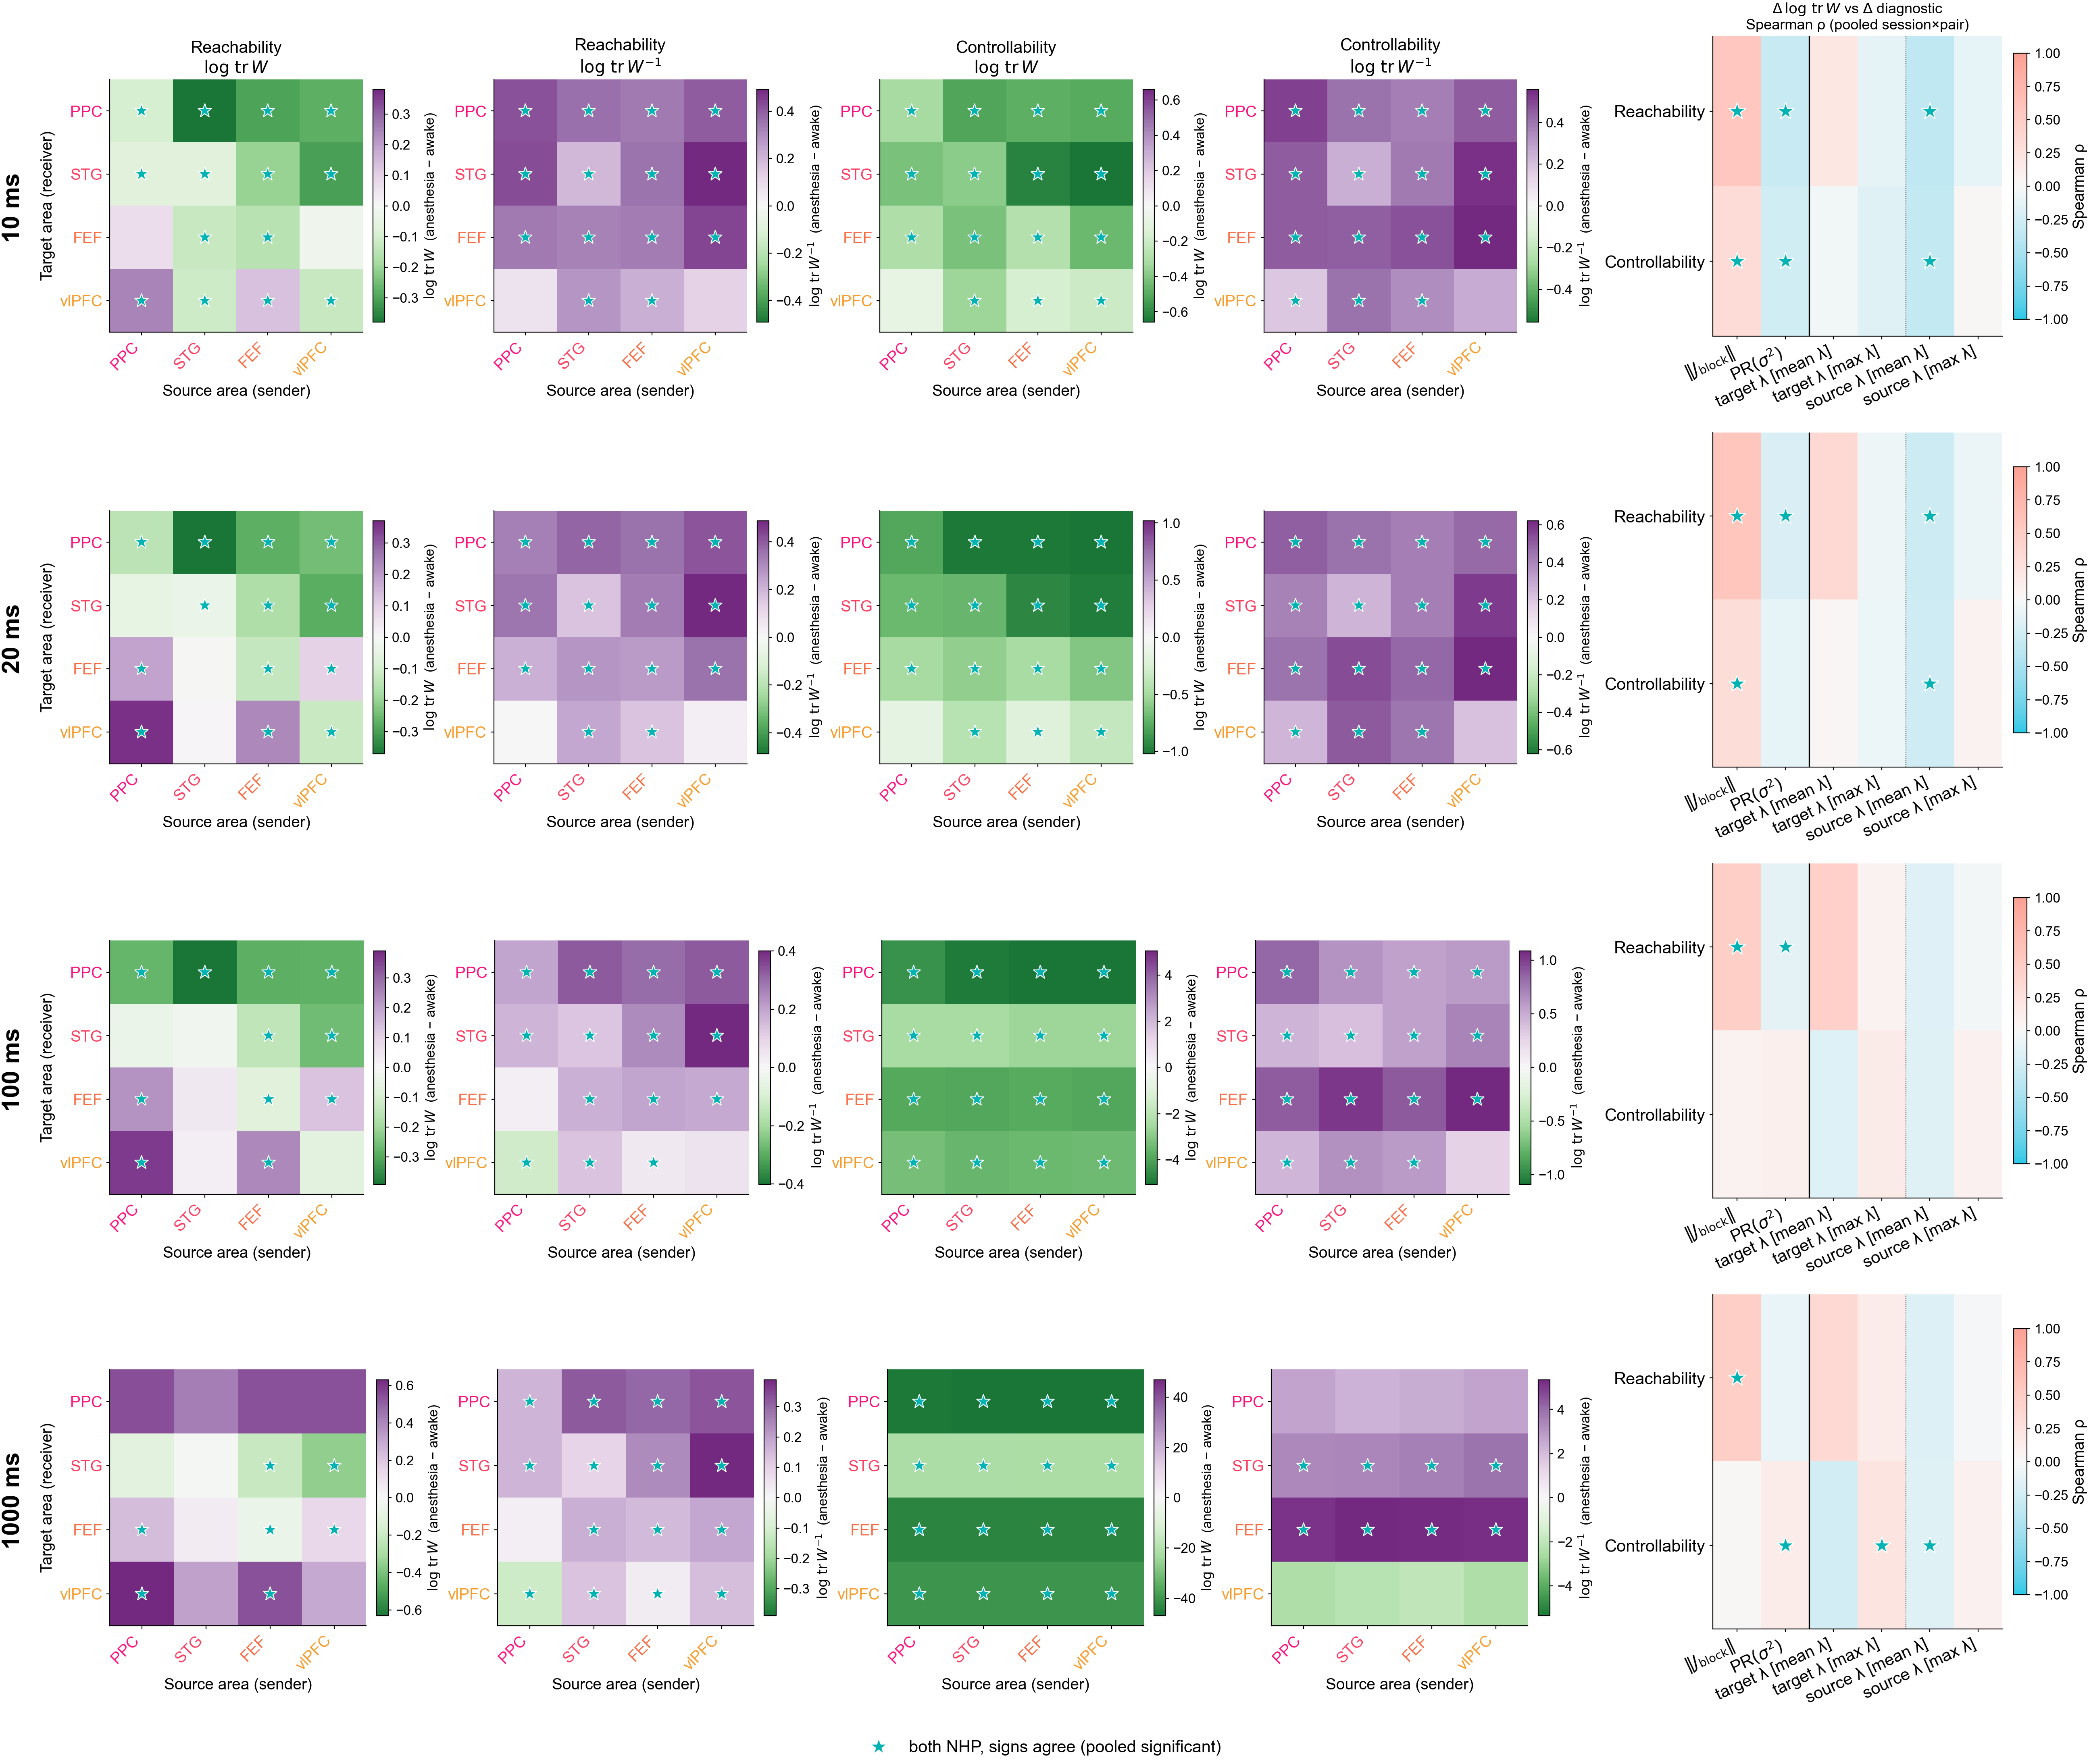
\includegraphics[width=\linewidth,height=0.78\textheight,keepaspectratio]{figures/interareal-control/fig_neural_control_horizons.png}
\caption[Interareal control summaries across integration horizons]{\textbf{Interareal control summaries across integration horizons} ($n=21$ sessions). Rows: gramian integration horizon ($10$, $20$, $100$, $1000\,\mathrm{ms}$). Columns 1--4: $4\!\times\!4$ source--target heatmaps of pooled anesthesia$-$awake differences in reachability $\log\mathrm{tr}\,\mathbf{W}$ and $\log\mathrm{tr}\,\mathbf{W}^{-1}$ and controllability $\log\mathrm{tr}\,\mathbf{W}$ and $\log\mathrm{tr}\,\mathbf{W}^{-1}$; teal stars mark cells passing the sign-agree $+$ BH-FDR gate at $q<0.05$ (same convention as Fig.~\ref{fig:interareal-control-neural-control}A,B). Column 5: Spearman correlation between the per-pair change in gramian $\log\mathrm{tr}\,\mathbf{W}$ and the change in block-norm, participation ratio, and source- and target-area Lyapunov exponents, with session-clustered permutation testing (same construction as Fig.~\ref{fig:interareal-control-neural-control}E), computed at that horizon. The $10\,\mathrm{ms}$ row reproduces the main-text summaries.}
\label{fig:interareal-control-gramian-horizons}
\end{figure}

At the control-relevant $10\,\mathrm{ms}$ horizon, as reported in the main text, anesthesia coherently shrinks reachability between areas: reachability $\log\mathrm{tr}\,\mathbf{W}$ decreased in $12/16$ directed pairs and the worst-case control cost $\log\mathrm{tr}\,\mathbf{W}^{-1}$ increased in $14/16$, while controllability $\log\mathrm{tr}\,\mathbf{W}$ decreased in $15/16$ pairs (sign-agree pooled Wilcoxon, BH-FDR $q<0.05$; Figure~\ref{fig:interareal-control-gramian-horizons}, top row). This coherent reachability reduction progressively dissolves as the horizon lengthens: the number of pairs with a significant reachability $\log\mathrm{tr}\,\mathbf{W}$ decrease falls from $12$ ($10\,\mathrm{ms}$) to $9$ ($20\,\mathrm{ms}$) to $7$ ($100\,\mathrm{ms}$) to $3$ ($1\,\mathrm{s}$), and by $1\,\mathrm{s}$ the pooled mean difference has reversed sign (pooled mean $\Delta=+0.22$, vs.\ $-0.11$ at $10\,\mathrm{ms}$). Controllability behaves oppositely: the trace decrease not only persists but amplifies monotonically with horizon (all $16/16$ pairs significant by $100\,\mathrm{ms}$; pooled mean $\Delta=-0.39,\,-0.65,\,-3.7,\,-38$ across the four horizons), as the longer integration window accumulates more of the within-target propagator relative to the bounded cross-area input.

The diagnostic correlations tell the same story from the explanatory side. At $10$--$20\,\mathrm{ms}$, the change in reachability tracks the change in cross-area coupling magnitude ($\Delta\|\mathbf{J}_{\mathrm{block}}\|$, $\rho=+0.56$), coupling dimensionality ($\Delta\mathrm{PR}(\sigma^{2})$, $\rho=-0.31$), and source-area stability ($\Delta$source-area $\lambda$, $\rho=-0.36$; all session-clustered permutation $p<0.05$). As the horizon lengthens, the source-area-$\lambda$ and participation-ratio associations vanish---neither survives the clustered-permutation test beyond $20\,\mathrm{ms}$---and the only correlate that remains stable across all four horizons is coupling magnitude ($\rho=+0.56,\,+0.57,\,+0.48,\,+0.47$). A target-area-$\lambda$ association emerges at the longer horizons but does not reach significance ($\rho=+0.45$ at $100\,\mathrm{ms}$, $p=0.08$). The explanatory weight thus migrates from the input coupling toward the target area's own dynamics as the integration window grows.

Together these trends indicate that the anesthesia-driven reachability reorganization reported in the chapter is a short-horizon, coupling-governed effect. Over longer windows the within-area state-transition propagator $\mathbf{\Phi}^{\alpha}\sim\exp(\mathbf{J}^{\alpha\to\alpha}\,t)$ (the intrinsic dynamics whose leading Lyapunov exponents are characterized in \S\ref{supp:interareal-control-lyap-extra}) increasingly dominates the gramian over the cross-area input term, reshaping the apparent reachability landscape (the sign reversal at $1\,\mathrm{s}$). At the same time, the destabilized anesthetic state drives the controllability ease even further down over long horizons. Crucially, the increased reachability capability under anesthesia is past the timescale on which one area can steer another before the target's own dynamics carry its state away: by the point at which intrinsic dynamics set the reachability landscape, the window for directed interareal control has effectively closed. The reachability disruption (reduced reachability under anesthesia, set by the interareal coupling) is the one visible at the short, functionally relevant horizon.

\FloatBarrier

\section{Proofs}\label{supp:interareal-control-proofs}

\subsection{Jacobian-parameterized time derivative}\label{supp:interareal-control-proof-Fjac}

The trick that makes JacobianODE estimation backpropagate cleanly through $\hat{\mathbf{J}}^\theta$ rather than through a separately-parameterized $\vb{f}$ is to express the instantaneous time derivative as a functional of the Jacobian alone, evaluated along a smooth path between two observed states. By the fundamental theorem of calculus along the trajectory,
\begin{equation}
\vb{x}(t)-\vb{x}(t_0) \;=\; \int_{t_0}^{t}\vb{f}(\vb{x}(s))\,ds.
\end{equation}
The conservativity-induced path-integral identity (Eq.~\ref{eq:interareal-control-pathint}) lets us replace each integrand $\vb{f}(\vb{x}(s))$ by $\vb{f}(\vb{x}(t))$ minus the path integral of $\mathbf{J}$ from $\vb{x}(s)$ to $\vb{x}(t)$, and solving the resulting linear relation for $\vb{f}(\vb{x}(t))$ gives the central proposition used throughout JacobianODE training.

\begin{proposition}[Jacobian-parameterized $\vb{f}$]\label{prop:supp-interareal-control-Fjac}
Given observed states $\vb{x}(t_0)$ and $\vb{x}(t)$ along a trajectory of $\dot{\vb{x}}=\vb{f}(\vb{x})$ with continuous Jacobian $\mathbf{J}=\nabla\vb{f}$, there exists a functional $\mathcal{F}$ of $\mathbf{J}$ alone such that
\begin{equation}
\mathcal{F}\!\left[\mathbf{J};\,\vb{x}(t_0),\vb{x}(t),t_0,t\right] \;=\; \vb{f}(\vb{x}(t)).
\end{equation}
Explicitly,
\begin{equation}
\boxed{\;\mathcal{F}\!\left[\mathbf{J};\,\vb{x}(t_0),\vb{x}(t),t_0,t\right] \;=\; \frac{\vb{x}(t)-\vb{x}(t_0)+G(t_0,t;\,\mathbf{J})}{t-t_0}\;}\label{eq:supp-interareal-control-Fjac}
\end{equation}
where
\begin{equation}
G(t_0,t;\,\mathbf{J}) \;=\; \int_{t_0}^{t}\!\int_{s}^{t} \mathbf{J}(\vb{c}_{s,t}(r))\,\vb{c}_{s,t}'(r)\,dr\,ds,\label{eq:supp-interareal-control-G}
\end{equation}
and $\vb{c}_{s,t}:[s,t]\to\mathbb{R}^{d}$ is any smooth curve with $\vb{c}_{s,t}(s)=\vb{x}(s)$ and $\vb{c}_{s,t}(t)=\vb{x}(t)$.
\end{proposition}

\begin{proof}
By the fundamental theorem of calculus along the trajectory,
\begin{equation}
\vb{x}(t)-\vb{x}(t_0) \;=\; \int_{t_0}^{t} \vb{f}(\vb{x}(s))\,ds. \label{eq:supp-interareal-control-ftc}
\end{equation}
By the row-conservativity path-integral identity, for each $s\in[t_0,t]$,
\begin{equation}
\vb{f}(\vb{x}(s)) \;=\; \vb{f}(\vb{x}(t)) \;-\; \int_{s}^{t} \mathbf{J}(\vb{c}_{s,t}(r))\,\vb{c}_{s,t}'(r)\,dr. \label{eq:supp-interareal-control-fpath}
\end{equation}
Substituting Eq.~\ref{eq:supp-interareal-control-fpath} into Eq.~\ref{eq:supp-interareal-control-ftc} and pulling $\vb{f}(\vb{x}(t))$ outside the now-trivial $s$-integral yields
\begin{equation}
\vb{x}(t)-\vb{x}(t_0) \;=\; (t-t_0)\,\vb{f}(\vb{x}(t)) \;-\; \underbrace{\int_{t_0}^{t}\!\int_{s}^{t} \mathbf{J}(\vb{c}_{s,t}(r))\,\vb{c}_{s,t}'(r)\,dr\,ds}_{G(t_0,t;\,\mathbf{J})}.
\end{equation}
Rearranging gives $\vb{f}(\vb{x}(t)) = \big[\vb{x}(t)-\vb{x}(t_0)+G(t_0,t;\,\mathbf{J})\big]/(t-t_0)$. \end{proof}

\begin{remark}
Equation~\ref{eq:supp-interareal-control-Fjac} is implemented in \texttt{JacobianODE/jacobians/jacobianODE.py}: the double integral $G$ uses a straight-line path $\vb{c}_{s,t}(r)=\vb{x}(s)+(r-s)(\vb{x}(t)-\vb{x}(s))/(t-s)$ with the trapezoid rule from \texttt{torchquad} (\texttt{N=20} subdivisions); the resulting estimate of $\vb{f}(\vb{x}(t))$ is then advanced one step by a standard ODE integrator (default: RK4 from \texttt{torchdiffeq}). Because $\mathcal{F}$ depends only on $\mathbf{J}$, all gradients backpropagate through $\hat{\mathbf{J}}^\theta$, and no separate $\vb{f}$-network is trained.
\end{remark}

\subsection{Invariance of the pairwise reachability Gramian trace under isometric direct-sum diffeomorphism}\label{supp:interareal-control-proof-gram-inv}

The pairwise reachability Gramian quantifies how strongly source area $\beta$ can drive target area $\alpha$ along the reference trajectory. We show that when the encoder respects the subsystem product structure---that is, each subsystem's latent coordinates depend only on that subsystem's observed coordinates---and is an isometry on each subsystem factor, the pairwise reachability Gramian computed in the latent is conjugate by an orthogonal map to the Gramian one would compute on the (unknown) data side. Hence the trace and the full eigenvalue spectrum are exactly preserved.

\paragraph{Setup.}
Let $\mathcal{M}=\mathcal{M}^1\times\cdots\times\mathcal{M}^K$ and $\widetilde{\mathcal{M}}=\widetilde{\mathcal{M}}^1\times\cdots\times\widetilde{\mathcal{M}}^K$ be Riemannian product manifolds with product metrics $g_{\mathcal{M}}=\bigoplus_{k}g_{\mathcal{M}}^{k}$ and $g_{\widetilde{\mathcal{M}}}=\bigoplus_{k}g_{\widetilde{\mathcal{M}}}^{k}$. Assume the encoder is a \emph{direct sum of diffeomorphisms}, with each area's encoded coordinates depending only on that area's observed coordinates---this is precisely the per-subsystem encoder construction of the Diffeomorphic-encoder subsection of the chapter Methods section, $\vb{z}=\vb{\Psi}(\tilde{\vb{x}})=[\vb{\Psi}^{1}(\tilde{\vb{x}}^{1});\,\ldots;\,\vb{\Psi}^{K}(\tilde{\vb{x}}^{K})]$,
\begin{equation}
\vb{\Psi}(\tilde{\vb{x}}^{1},\ldots,\tilde{\vb{x}}^{K}) \;=\; \bigl(\vb{\Psi}^{1}(\tilde{\vb{x}}^{1}),\,\ldots,\,\vb{\Psi}^{K}(\tilde{\vb{x}}^{K})\bigr),
\end{equation}
with each $\vb{\Psi}^{k}$ an isometric diffeomorphism. Then $\vb{\Psi}$ is itself an isometry, and its differential is block-diagonal:
\begin{equation}
D\vb{\Psi}(\tilde{\vb{x}}) \;=\; D\vb{\Psi}^{1}(\tilde{\vb{x}}^{1})\,\oplus\,\cdots\,\oplus\,D\vb{\Psi}^{K}(\tilde{\vb{x}}^{K}).\label{eq:supp-interareal-control-blockdiagD}
\end{equation}
We will write $D\vb{\Psi}^{\alpha}_{t}\triangleq D\vb{\Psi}^{\alpha}(\tilde{\vb{x}}^{\alpha}(t))$ for short, and similarly for the other subsystems. All adjoints $(\cdot)^{*}$ below are taken with respect to the metric on each side. We write $\mathbf{J}^{\beta\to\alpha}(\tilde{\vb{x}})$ for the data-side cross-area Jacobian block (rows of area $\alpha$, columns of area $\beta$), $\widetilde{\mathbf{J}}^{\beta\to\alpha}(\vb{z})$ for its latent-side counterpart, $\mathbf{\Phi}^{\alpha}(t_{1},\tau)$ for the within-$\alpha$ state-transition operator under $\mathbf{J}^{\alpha\to\alpha}$, and $\widetilde{\mathbf{\Phi}}^{\alpha}(t_{1},\tau)$ for its latent counterpart. Following the pairwise tangent-space equation in \S\ref{sec:interareal-control-methods},
\begin{equation}
\mathbf{W}_{r}^{\beta\to\alpha}(t_{0},t_{1}) \;=\; \int_{t_{0}}^{t_{1}} \mathbf{\Phi}^{\alpha}(t_{1},\tau)\,\mathbf{J}^{\beta\to\alpha}(\tilde{\vb{x}}(\tau))\,[\mathbf{J}^{\beta\to\alpha}(\tilde{\vb{x}}(\tau))]^{*}\,[\mathbf{\Phi}^{\alpha}(t_{1},\tau)]^{*}\,d\tau,\label{eq:supp-interareal-control-Wreach}
\end{equation}
and analogously $\widetilde{\mathbf{W}}_{r}^{\beta\to\alpha}(t_{0},t_{1})$ with the tilde objects.

\begin{theorem}[Spectral invariance of the pairwise reachability Gramian]\label{thm:supp-interareal-control-gram-inv}
Under the setup above, for any pair $(\alpha,\beta)\in\{1,\ldots,K\}^{2}$ with $\alpha\neq\beta$, the pairwise reachability Gramian on the latent is conjugate to the pairwise reachability Gramian on the data by an orthogonal map at the final time:
\begin{equation}
\widetilde{\mathbf{W}}_{r}^{\beta\to\alpha}(t_{0},t_{1}) \;=\; D\vb{\Psi}^{\alpha}_{t_{1}}\,\mathbf{W}_{r}^{\beta\to\alpha}(t_{0},t_{1})\,(D\vb{\Psi}^{\alpha}_{t_{1}})^{-1}.\label{eq:supp-interareal-control-gram-conj}
\end{equation}
In particular,
\begin{equation}
\operatorname{tr}\widetilde{\mathbf{W}}_{r}^{\beta\to\alpha}(t_{0},t_{1}) \;=\; \operatorname{tr}\mathbf{W}_{r}^{\beta\to\alpha}(t_{0},t_{1}),
\end{equation}
and the full eigenvalue spectrum---including $\lambda_{\min}$---is preserved.
\end{theorem}

\begin{proof}
Each $\vb{\Psi}^{k}$ is an isometry, so $D\vb{\Psi}^{k}$ is orthogonal:
\begin{equation}
(D\vb{\Psi}^{k})^{*}=(D\vb{\Psi}^{k})^{-1}\quad\text{for all }k\in\{1,\ldots,K\}.
\end{equation}
The block-diagonal structure of Eq.~\ref{eq:supp-interareal-control-blockdiagD} means that differentiating $D\vb{\Psi}^{\alpha}(\tilde{\vb{x}}^{\alpha})$ with respect to $\tilde{\vb{x}}^{\beta}$ for $\beta\neq\alpha$ gives zero, so the chain rule applied to the cross-area block of the Jacobian yields a clean conjugation \emph{between} the two subsystem factors, with no $D^{2}\vb{\Psi}$ correction term:
\begin{equation}
\widetilde{\mathbf{J}}^{\beta\to\alpha}(\vb{z}) \;=\; D\vb{\Psi}^{\alpha}(\tilde{\vb{x}}^{\alpha})\,\mathbf{J}^{\beta\to\alpha}(\tilde{\vb{x}})\,(D\vb{\Psi}^{\beta}(\tilde{\vb{x}}^{\beta}))^{-1}.\label{eq:supp-interareal-control-Jconj}
\end{equation}
Taking the adjoint of Eq.~\ref{eq:supp-interareal-control-Jconj} and using orthogonality,
\begin{equation}
[\widetilde{\mathbf{J}}^{\beta\to\alpha}(\vb{z})]^{*} \;=\; D\vb{\Psi}^{\beta}(\tilde{\vb{x}}^{\beta})\,[\mathbf{J}^{\beta\to\alpha}(\tilde{\vb{x}})]^{*}\,(D\vb{\Psi}^{\alpha}(\tilde{\vb{x}}^{\alpha}))^{-1}.
\end{equation}
So the $\beta$-side factors collapse in the symmetric product:
\begin{equation}
\widetilde{\mathbf{J}}^{\beta\to\alpha}\,[\widetilde{\mathbf{J}}^{\beta\to\alpha}]^{*} \;=\; D\vb{\Psi}^{\alpha}\,\mathbf{J}^{\beta\to\alpha}\,[\mathbf{J}^{\beta\to\alpha}]^{*}\,(D\vb{\Psi}^{\alpha})^{-1}. \label{eq:supp-interareal-control-Bsym}
\end{equation}
The within-$\alpha$ state-transition operator transforms similarly: from $\delta\vb{z}^{\alpha}(t)=D\vb{\Psi}^{\alpha}_{t}\,\delta\tilde{\vb{x}}^{\alpha}(t)$ and the definition of $\mathbf{\Phi}^{\alpha}$,
\begin{equation}
\widetilde{\mathbf{\Phi}}^{\alpha}(t_{1},\tau) \;=\; D\vb{\Psi}^{\alpha}_{t_{1}}\,\mathbf{\Phi}^{\alpha}(t_{1},\tau)\,(D\vb{\Psi}^{\alpha}_{\tau})^{-1},\label{eq:supp-interareal-control-Phiconj}
\end{equation}
and analogously for the adjoint $[\widetilde{\mathbf{\Phi}}^{\alpha}(t_{1},\tau)]^{*}=D\vb{\Psi}^{\alpha}_{\tau}\,[\mathbf{\Phi}^{\alpha}(t_{1},\tau)]^{*}\,(D\vb{\Psi}^{\alpha}_{t_{1}})^{-1}$. Substituting Eq.~\ref{eq:supp-interareal-control-Bsym} and Eq.~\ref{eq:supp-interareal-control-Phiconj} into the integrand of $\widetilde{\mathbf{W}}_{r}^{\beta\to\alpha}$,
\begin{align}
&\widetilde{\mathbf{\Phi}}^{\alpha}(t_{1},\tau)\,\widetilde{\mathbf{J}}^{\beta\to\alpha}\,[\widetilde{\mathbf{J}}^{\beta\to\alpha}]^{*}\,[\widetilde{\mathbf{\Phi}}^{\alpha}(t_{1},\tau)]^{*} \nonumber\\
&\quad=\; D\vb{\Psi}^{\alpha}_{t_{1}}\,\Bigl[\mathbf{\Phi}^{\alpha}(t_{1},\tau)\,\mathbf{J}^{\beta\to\alpha}\,[\mathbf{J}^{\beta\to\alpha}]^{*}\,[\mathbf{\Phi}^{\alpha}(t_{1},\tau)]^{*}\Bigr]\,(D\vb{\Psi}^{\alpha}_{t_{1}})^{-1},
\end{align}
where every intermediate $D\vb{\Psi}^{\alpha}_{\tau}$ pair cancels: each $D\vb{\Psi}^{\alpha}_{\tau}$ appears next to its inverse, and likewise for the $D\vb{\Psi}^{\beta}_{\tau}$ pair that hid inside the symmetric product Eq.~\ref{eq:supp-interareal-control-Bsym}. Integrating over $\tau$ and pulling the $\tau$-independent outer factors out gives Eq.~\ref{eq:supp-interareal-control-gram-conj}. Trace and eigenvalues are invariant under conjugation by an invertible operator. \end{proof}

\begin{remark}
The proof extends pointwise to any number of subsystems $K\geq 2$, with the only requirement being that the encoder respect the subsystem product structure (each $\vb{\Psi}^{k}$ acts only on $\tilde{\vb{x}}^{k}$). It also extends to the controllability Gramian by replacing $\mathbf{\Phi}^{\alpha}(t_{1},\tau)$ with $\mathbf{\Phi}^{\alpha}(t_{0},\tau)$ throughout. The hypothesis that each $\vb{\Psi}^{k}$ is an isometry is stronger than what the NICE--Cayley encoder of \S\ref{supp:interareal-control-encoder-details} guarantees by construction (the encoder is volume-preserving but not in general isometric); we therefore present the reachability and controllability log-trace summaries reported in the chapter as invariants up to encoder-induced similarity, which is what their trace summaries measure. The metric-adjusted Gramian construction of \S\ref{supp:interareal-control-gramian-metric} provides one route to mitigate the residual mismatch by re-weighting the input matrix by the inverse encoder Jacobian on the source-area input space.
\end{remark}

\subsection{Bounded error under generalized teacher forcing}\label{supp:interareal-control-proof-gtf}

Generalized teacher forcing (GTF)~\cite{Hess2023-kp} stabilizes recursive prediction by partially anchoring the rollout to the true trajectory. The strength of anchoring is a scalar $\alpha\in[0,1]$: the input to the next-step network at time $t$ is the convex combination
\begin{equation}
\tilde{\vb{x}}_{t} \;=\; \alpha\,\vb{x}_{t}\;+\;(1-\alpha)\,\hat{\vb{x}}_{t}, \qquad \tilde{\vb{x}}_{t+1}=\hat{F}(\tilde{\vb{x}}_{t}),
\end{equation}
where $\vb{x}_{t}$ is the true state, $\hat{\vb{x}}_{t}$ is the (potentially drifting) recursive prediction, and $\hat{F}$ is the learned one-step update. $\alpha=1$ recovers full teacher forcing; $\alpha=0$ recovers free-running prediction.

\begin{lemma}[Asymptotic bound on the product of one-step generators]\label{lem:supp-interareal-control-lyap-prod}
For every $\epsilon>0$ there exists $C\in\mathbb{R}_{+}$ such that for all $T\geq 1$,
\begin{equation}
\Bigl\|\prod_{t=0}^{T-1} e^{\mathbf{J}_{T-t}\Delta t}\Bigr\|_{2} \;\leq\; C\,\bigl(e^{\lambda_{\max}+\epsilon}\bigr)^{T},
\end{equation}
where $\lambda_{\max}=\lim_{T\to\infty}\frac{1}{T}\log\|\mathcal{G}_{T}\|_{2}$ is the maximum Lyapunov exponent of the linearized system along the trajectory and $\mathcal{G}_{T}=\prod_{t=0}^{T-1}e^{\mathbf{J}_{T-t}\Delta t}$.
\end{lemma}

\begin{proof}
By the definition of the maximum Lyapunov exponent, for every $\epsilon>0$ there exists $N$ such that for all $T>N$, $\frac{1}{T}\log\|\mathcal{G}_{T}\|_{2} < \lambda_{\max}+\epsilon$, which rearranges to
\begin{equation}
\|\mathcal{G}_{T}\|_{2} \;<\; e^{T(\lambda_{\max}+\epsilon)} \;=\; \bigl(e^{\lambda_{\max}+\epsilon}\bigr)^{T}.
\end{equation}
For the pre-asymptotic regime $1\leq T\leq N$, the sequence consists of finitely many bounded matrix products, so there exists $C\in\mathbb{R}_{+}$ such that $\|\mathcal{G}_{T}\|_{2}\leq C\bigl(e^{\lambda_{\max}+\epsilon}\bigr)^{T}$ for all $1\leq T\leq N$. Taking the larger of the two constants establishes the claim. \end{proof}

\begin{proposition}[Bounded error under GTF; cf.~\cite{Hess2023-kp}]\label{prop:supp-interareal-control-gtf}
Let $\hat{F}$ be the learned one-step update with bounded one-step approximation error, $\|\hat{F}(\vb{x}_{t})-F(\vb{x}_{t})\|_{2}\leq L$ for some $L\in\mathbb{R}_{+}$, and let the GTF strength satisfy
\begin{equation}
\alpha \;>\; 1 - e^{-\lambda_{\max}}.\label{eq:supp-interareal-control-gtf-bound}
\end{equation}
Then the prediction error $\vb{e}_{T}=\hat{\vb{x}}_{T}-\vb{x}_{T}$ remains bounded for all $T$.
\end{proposition}

\begin{proof}
Define $\delta_{t}=\hat{F}(\vb{x}_{t})-F(\vb{x}_{t})$ (one-step model error). Note that
\begin{equation}
\tilde{\vb{x}}_{t} \;=\; \alpha\,\vb{x}_{t}+(1-\alpha)\,\hat{\vb{x}}_{t} \;=\; \alpha\,\vb{x}_{t}+(1-\alpha)(\vb{x}_{t}+\vb{e}_{t}) \;=\; \vb{x}_{t}+(1-\alpha)\,\vb{e}_{t}.
\end{equation}
The error propagates as
\begin{align}
\vb{e}_{t+1} &= \hat{F}(\tilde{\vb{x}}_{t})-F(\vb{x}_{t}) \\
&= \bigl[\hat{F}(\tilde{\vb{x}}_{t})-\hat{F}(\vb{x}_{t})\bigr]+\bigl[\hat{F}(\vb{x}_{t})-F(\vb{x}_{t})\bigr] \\
&= \bigl[\hat{F}(\vb{x}_{t}+(1-\alpha)\vb{e}_{t})-\hat{F}(\vb{x}_{t})\bigr]+\delta_{t}.
\end{align}
Linearizing $\hat{F}$ about $\vb{x}_{t}$ (which is valid for sufficiently small $\vb{e}_{t}$),
\begin{equation}
\vb{e}_{t+1} \;\approx\; e^{\mathbf{J}_{t}\Delta t}\,(1-\alpha)\,\vb{e}_{t} \;+\; \delta_{t},
\end{equation}
where $\mathbf{J}_{t}=\nabla\hat{F}(\vb{x}_{t})/\Delta t$ in the continuous-time interpretation (or simply the one-step linearization in the discrete formulation). This recursion has solution
\begin{equation}
\vb{e}_{T} \;=\; \sum_{k=0}^{T-2} (1-\alpha)^{T-1-k}\Bigl(\prod_{t=k+1}^{T-1} e^{\mathbf{J}_{T-t}\Delta t}\Bigr)\,\delta_{k},
\end{equation}
with norm bound
\begin{equation}
\|\vb{e}_{T}\|_{2} \;\leq\; \sum_{k=0}^{T-2} (1-\alpha)^{T-1-k}\,\Bigl\|\prod_{t=k+1}^{T-1} e^{\mathbf{J}_{T-t}\Delta t}\Bigr\|_{2}\,\|\delta_{k}\|_{2}.
\end{equation}
Using $\|\delta_{k}\|_{2}\leq L$ and Lemma~\ref{lem:supp-interareal-control-lyap-prod},
\begin{equation}
\|\vb{e}_{T}\|_{2} \;\leq\; L\,C \sum_{k=0}^{T-2} \bigl[(1-\alpha)\,e^{\lambda_{\max}}\bigr]^{T-1-k} \;=\; L\,C \sum_{j=1}^{T-1}\bigl[(1-\alpha)\,e^{\lambda_{\max}}\bigr]^{j}.
\end{equation}
The geometric series on the right converges as $T\to\infty$ iff $(1-\alpha)\,e^{\lambda_{\max}}<1$, which is equivalent to Eq.~\ref{eq:supp-interareal-control-gtf-bound}. Under this condition, $\|\vb{e}_{T}\|_{2}\leq LC\,(1-\alpha)e^{\lambda_{\max}}/[1-(1-\alpha)e^{\lambda_{\max}}]$ uniformly in $T$. \end{proof}

\begin{remark}
The bound is tight in the sense that for $\alpha<1-e^{-\lambda_{\max}}$ the geometric series diverges and the error grows exponentially; the threshold $\alpha^{\star}=1-e^{-\lambda_{\max}}$ is therefore the minimum GTF strength that ensures bounded recursive prediction in the linearized regime. In practice we use $\alpha_{\mathrm{teacher\ forcing}}\in[\alpha_{\min},1]$ annealed over training (\S\ref{supp:interareal-control-gtf-impl}); both the per-rollout maximum effective $\lambda_{\max}$ (via the learned Jacobians along the reference trajectory) and the geometric series prefactor enter directly into the validity of the bound.
\end{remark}

\section{Modeling details}\label{supp:interareal-control-modeling}

\subsection{Diffeomorphic encoder}\label{supp:interareal-control-encoder-details}

\subsubsection{Delay embedding}\label{supp:interareal-control-delay-embed}

For each subsystem $k\in\{1,\ldots,K\}$, the per-subsystem observation $\vb{x}^{k}(t)\in\mathbb{R}^{d_{\mathrm{obs}}^{k}}$ is stacked with $n_{d}$ delayed copies at unit stride ($\tau\Delta t=\Delta t$):
\begin{equation}
\tilde{\vb{x}}^{k}(t) \;=\; \bigl[\vb{x}^{k}(t);\,\vb{x}^{k}(t-\Delta t);\,\ldots;\,\vb{x}^{k}(t-(n_{d}-1)\Delta t)\bigr] \;\in\; \mathbb{R}^{n_{d} d_{\mathrm{obs}}^{k}}.
\end{equation}
The full delay-embedded observation is the concatenation $\tilde{\vb{x}}(t)=[\tilde{\vb{x}}^{1}(t);\,\ldots;\,\tilde{\vb{x}}^{K}(t)]\in\mathbb{R}^{d'}$ with $d'=n_{d}\sum_{k}d_{\mathrm{obs}}^{k}$, ordered most-recent-first within each per-subsystem block. The choice of $n_{d}$ is a per-session sweep variable for the neural data. In practice, we take $\tau\Delta t=\Delta t$ which avoids the dimensionality blow-up of larger strides. For the propofol cohort, $n_{d}\in\{5,10,15\}$ was searched per session and per area (the per-area block size is $n_{d}\cdot 64$ for the typical 64-channel block).

\subsubsection{Additive coupling layers}\label{supp:interareal-control-additive-coupling}

Each additive coupling layer~\cite{Dinh2014-lx} acts on $\vb{y}\in\mathbb{R}^{n}$ by an even/odd channel split $\vb{y}=(\vb{a},\vb{b})$ with $\vb{a},\vb{b}\in\mathbb{R}^{n/2}$ and applies
\begin{equation}
\vb{a}' = \vb{a},\qquad \vb{b}' = \vb{b}+\vb{m}_{\vartheta}(\vb{a},\vb{c}),
\end{equation}
where $\vb{m}_{\vartheta}:\mathbb{R}^{n/2}\!\times\!\mathbb{R}^{d_{c}}\!\to\!\mathbb{R}^{n/2}$ is a conditioner MLP and $\vb{c}$ is a (per-trial, per-batch) condition vector (binary $\{-1,+1\}$ for awake-vs-anesthesia). The layer Jacobian is
\begin{equation}
\frac{\partial(\vb{a}',\vb{b}')}{\partial(\vb{a},\vb{b})} \;=\; \begin{bmatrix}\mathbf{I}&\mathbf{0}\\ \nabla_{\!\vb{a}}\vb{m}_{\vartheta}&\mathbf{I}\end{bmatrix},
\end{equation}
which is unit-triangular: $\det=1$ identically, regardless of $\vb{m}_{\vartheta}$, $\vb{a}$, or $\vb{c}$. The layer is exactly invertible by $\vb{a}=\vb{a}'$, $\vb{b}=\vb{b}'-\vb{m}_{\vartheta}(\vb{a}',\vb{c})$ in one forward pass.

\subsubsection{Cayley orthogonal mixers}\label{supp:interareal-control-cayley}

Between consecutive coupling layers we insert a learnable rotation $\mathbf{Q}\in\mathrm{SO}(n)$ parameterized by the Cayley transform of a learnable skew-symmetric matrix $\mathbf{A}=-\mathbf{A}^{\!\top}\in\mathbb{R}^{n\times n}$:
\begin{equation}
\mathbf{Q} \;=\; (\mathbf{I}-\mathbf{A})\,(\mathbf{I}+\mathbf{A})^{-1}.
\end{equation}
\begin{lemma}\label{lem:supp-interareal-control-cayley}
For any skew-symmetric $\mathbf{A}$ with $-1\notin\mathrm{spec}(\mathbf{A})$, $\mathbf{Q}$ is orthogonal with $\det\mathbf{Q}=+1$.
\end{lemma}
\begin{proof}
$\mathbf{Q}^{\!\top}\mathbf{Q}=(\mathbf{I}+\mathbf{A})^{-\top}(\mathbf{I}-\mathbf{A})^{\!\top}(\mathbf{I}-\mathbf{A})(\mathbf{I}+\mathbf{A})^{-1}=(\mathbf{I}-\mathbf{A})^{-1}(\mathbf{I}+\mathbf{A})(\mathbf{I}-\mathbf{A})(\mathbf{I}+\mathbf{A})^{-1}=\mathbf{I}$ since $(\mathbf{I}-\mathbf{A})$ and $(\mathbf{I}+\mathbf{A})$ share an eigenbasis (commute) and cancel pairwise. The eigenvalues of $\mathbf{A}$ are purely imaginary in conjugate pairs $\pm i\omega_{k}$, so the eigenvalues of $\mathbf{Q}$ are $(1-i\omega_{k})/(1+i\omega_{k})$---complex of unit modulus in conjugate pairs---and their product is $+1$.
\end{proof}

Implementation uses \texttt{torch.linalg.solve(I$-$A, I$+$A)} rather than an explicit inverse for stability. The skew parameter is built from the strict upper triangle of a free parameter $\mathbf{U}\in\mathbb{R}^{n\times n}$ via $\mathbf{A}=\mathrm{striu}(\mathbf{U})-\mathrm{striu}(\mathbf{U})^{\!\top}$ (the lower triangle and diagonal of $\mathbf{U}$ are unused, and the operation projects to the skew subspace automatically).

\subsubsection{Volume-preserving composition and identity-at-initialization}\label{supp:interareal-control-composition}

Let $\vb{\Psi}^{k}=\mathbf{Q}^{k}_{L}\circ\mathcal{C}^{k}_{L}\circ\cdots\circ\mathbf{Q}^{k}_{1}\circ\mathcal{C}^{k}_{1}$ denote the per-subsystem encoder (composition of $L$ additive coupling layers $\mathcal{C}^{k}_{\ell}$ with Cayley mixers $\mathbf{Q}^{k}_{\ell}$). By the chain rule and Lemma~\ref{lem:supp-interareal-control-cayley},
\begin{equation}
\det\nabla\vb{\Psi}^{k}(\vb{y}) \;=\; \prod_{\ell=1}^{L}\det\nabla\mathbf{Q}^{k}_{\ell}\cdot\det\nabla\mathcal{C}^{k}_{\ell}(\vb{z}^{k}_{\ell}) \;=\; \prod_{\ell=1}^{L}(+1)\cdot(+1) \;=\; +1,
\end{equation}
so $|\det\nabla\vb{\Psi}^{k}|\equiv 1$ everywhere on its domain, and each $\vb{\Psi}^{k}$ is a $C^{\infty}$ diffeomorphism on $\mathbb{R}^{n_{d}d_{\mathrm{obs}}^{k}}$. The full encoder $\vb{\Psi}=(\vb{\Psi}^{1},\ldots,\vb{\Psi}^{K})$ inherits these properties on $\mathbb{R}^{d'}$ and respects the subsystem product structure required by Theorem~\ref{thm:supp-interareal-control-gram-inv}.

\emph{Identity-at-initialization.} We zero-initialize the last linear layer of every conditioner MLP, which makes $\vb{m}_{\vartheta}(\cdot,\cdot)\equiv\vb{0}$ at step 0; every coupling layer is then the identity map. We zero-initialize every skew parameter $\mathbf{U}=\vb{0}$, which gives $\mathbf{Q}=\mathbf{I}$. A final fixed permutation is appended whose composition with the random per-layer permutations equals the identity, so the entire encoder reduces to $\vb{\Psi}=\mathrm{id}$ at step 0. Training therefore departs from the trivial identity-reconstruction solution only as the trajectory and loop-closure losses begin to drive learning, which empirically gives the LR schedule a clean reconstruction-floor starting point.

\subsubsection{Zero-padded reconstruction loss}\label{supp:interareal-control-zero-pad-rec}

The encoder is dimension-preserving on $\mathbb{R}^{d'}$, but the intrinsic dimensionality of the dynamics is much smaller. The latent is partitioned as $\vb{z}=[\vb{z}_{\mathrm{dyn}};\vb{z}_{\mathrm{null}}]\in\mathbb{R}^{d_{\mathrm{dyn}}}\oplus\mathbb{R}^{d_{\mathrm{null}}}$ with $d_{\mathrm{null}}=d'-d_{\mathrm{dyn}}$. The dynamic-subspace dimension $d_{\mathrm{dyn}}$ is fixed per session by a PCA on the delay-embedded training data at variance threshold $0.99$ (per-area block selection; the resulting $d_{\mathrm{dyn}}^{k}$ values are concatenated to define the projection $P_{\mathrm{dyn}}=\mathrm{diag}(\mathbf{I}_{d_{\mathrm{dyn}}},\,\mathbf{0}_{d_{\mathrm{null}}})$). All decoder calls in the model use the zero-padded latent $[P_{\mathrm{dyn}}\vb{z};\,\vb{0}]$ rather than $\vb{z}$ itself, so any information that lives in $\vb{z}_{\mathrm{null}}$ is ignored on the round-trip. The reconstruction loss (Eq.~\ref{eq:interareal-control-reconstruction-loss}) therefore takes the form
\begin{equation}
\mathcal{L}_{\mathrm{rec}}(\theta_{\Psi};\vb{x}) \;=\; \mathbb{E}_{t}\Bigl[\bigl\|\vb{\Psi}^{-1}\bigl([P_{\mathrm{dyn}}\vb{\Psi}(\tilde{\vb{x}}(t));\,\vb{0}]\bigr)-\tilde{\vb{x}}(t)\bigr\|_{2}^{2}\Bigr],
\end{equation}
penalizing the round-trip error under the zero-padded forward map. Since $\vb{\Psi}$ is volume-preserving, every information-bearing dimension of the input \emph{must} survive somewhere in $\vb{z}$; the dynamic/null split together with the zero-padded round-trip squeeze incentivizes the encoder to concentrate the dynamics-relevant information into $\vb{z}_{\mathrm{dyn}}$ and dump dynamics-irrelevant content (noise, off-manifold variability) into $\vb{z}_{\mathrm{null}}$, where it cannot interfere with the Jacobian-MLP fit.

\subsubsection{Induced Riemannian metric on the latent}\label{supp:interareal-control-induced-metric}

The encoder $\vb{\Psi}$ pulls the (assumed-Euclidean) data-side metric on $\tilde{\vb{x}}$ forward to a Riemannian metric on $\vb{z}$:
\begin{equation}
\mathbf{R}(\vb{z}) \;=\; \bigl[\nabla\vb{\Psi}^{-1}(\vb{z})\bigr]^{\!\top}\,\bigl[\nabla\vb{\Psi}^{-1}(\vb{z})\bigr] \;=\; \bigl[D\vb{\Psi}(\vb{\Psi}^{-1}(\vb{z}))\,D\vb{\Psi}(\vb{\Psi}^{-1}(\vb{z}))^{\!\top}\bigr]^{-1}.
\end{equation}
Equivalently, in encoder-Jacobian form, $\mathbf{R}^{-1}(\vb{z})=\mathbf{J}_{E}(\tilde{\vb{x}})\,\mathbf{J}_{E}(\tilde{\vb{x}})^{\!\top}$ with $\mathbf{J}_{E}=D\vb{\Psi}$ evaluated at $\tilde{\vb{x}}=\vb{\Psi}^{-1}(\vb{z})$. Volume preservation gives $\det\mathbf{R}\equiv 1$, so the induced metric has unit determinant everywhere; isotropy of $\mathbf{R}$ (i.e., $\mathbf{R}\equiv\mathbf{I}$) corresponds exactly to the encoder being a Riemannian isometry, which is the hypothesis of Theorem~\ref{thm:supp-interareal-control-gram-inv}. In practice, while we don't enforce isometry, we find that volume preservation is sufficient to reproduce relative changes in the Gramians on the synthetic systems.

\subsubsection{Encoder geometry diagnostics: rotation angle, Haar reference, and geodesic distance}\label{supp:interareal-control-encoder-geom}

Two scalar diagnostics summarize how strongly the trained encoder rotates and warps the latent geometry (Figure~\ref{fig:interareal-control-neural-lyap}B,C).

\paragraph{Per-layer rotation angle.} Each Cayley mixer $\mathbf{Q}^{k}_{\ell}\in\mathrm{SO}(n)$ (\S\ref{supp:interareal-control-cayley}) has eigenvalues in unit-modulus conjugate pairs $e^{\pm i\theta_{m}}$ with $\theta_{m}=2\arctan\omega_{m}$, where $\pm i\omega_{m}$ are the purely imaginary eigenvalues of its skew generator $\mathbf{A}^{k}_{\ell}$. We summarize the rotation of a single mixer by the mean over modes of the absolute eigen-angle,
\begin{equation}
\bar\theta(\mathbf{Q}) \;=\; \frac{1}{n}\sum_{m=1}^{n}\bigl|\arg\lambda_{m}(\mathbf{Q})\bigr| \;\in\;[0,\pi],\label{eq:supp-interareal-control-rot-angle}
\end{equation}
computed numerically as the mean of $|\mathrm{angle}(\mathrm{eigvals}(\mathbf{Q}))|$; $\bar\theta=0$ is the identity (no mixing). Figure~\ref{fig:interareal-control-neural-lyap}B reports this per Cayley mixer index $\ell$ through encoder depth, both for the individual mixers $\mathbf{Q}^{k}_{\ell}$ and for the cumulative composite rotation $\mathbf{Q}^{k}_{\ell}\cdots\mathbf{Q}^{k}_{1}$ (the net rotation accrued up to depth $\ell$), averaged over the per-area blocks $k$.

\paragraph{Haar $\mathrm{SO}(n)$ reference.} To calibrate the rotation-angle scale we compare against the angle a \emph{maximally mixed} rotation would produce: a matrix drawn uniformly from $\mathrm{SO}(n)$ under the Haar measure. We sample $\mathbf{G}\sim\mathcal{N}(0,1)^{n\times n}$, take its QR decomposition $\mathbf{G}=\mathbf{Q}\mathbf{R}$, fix the column signs by $\mathbf{Q}\leftarrow\mathbf{Q}\,\mathrm{diag}(\mathrm{sgn}(\mathrm{diag}\,\mathbf{R}))$ (which makes the draw exactly Haar-uniform on $\mathrm{O}(n)$), and negate the first column whenever $\det\mathbf{Q}<0$ to land on the $\mathrm{SO}(n)$ component. The reference is $\bar\theta(\mathbf{Q})$ of Eq.~\ref{eq:supp-interareal-control-rot-angle} averaged over many such draws and over the per-area block dimensions $n$. The trained mixers sit between the identity ($\bar\theta=0$) and this Haar saturation level, quantifying how far each layer has rotated relative to a fully randomized rotation of the same dimension.

\paragraph{Geodesic distance of the induced metric to the identity.} The induced metric $\mathbf{R}(\vb{z})$ of \S\ref{supp:interareal-control-induced-metric} (equivalently its inverse $\mathbf{G}=\mathbf{J}_{E}\mathbf{J}_{E}^{\!\top}$) is symmetric positive definite (SPD). The natural distance between SPD matrices is the affine-invariant Riemannian (geodesic) distance, whose value relative to the identity is
\begin{equation}
d(\mathbf{I},\mathbf{G}) \;=\; \bigl\|\log\mathbf{G}\bigr\|_{F} \;=\; \Bigl(\sum_{m}\bigl(\log\lambda_{m}(\mathbf{G})\bigr)^{2}\Bigr)^{1/2},\label{eq:supp-interareal-control-spd-geo}
\end{equation}
where $\lambda_{m}(\mathbf{G})$ are the eigenvalues of $\mathbf{G}$ and $\log$ is the matrix logarithm; this is invariant to the choice of $\mathbf{R}$ versus $\mathbf{R}^{-1}=\mathbf{G}$ since $\log\mathbf{R}^{-1}=-\log\mathbf{G}$. Writing $\lambda_{m}(\mathbf{G})=\sigma_{m}^{2}$ in terms of the singular values $\sigma_{m}$ of the composite encoder Jacobian $\mathbf{J}_{E}$ along the $d_{\mathrm{dyn}}$ retained (dynamic-subspace) modes, $\log\lambda_{m}=2\log\sigma_{m}$. We report the per-mode root-mean-square normalization of Eq.~\ref{eq:supp-interareal-control-spd-geo} (dividing the Frobenius norm by $\sqrt{d_{\mathrm{dyn}}}$ so the scale is $O(1)$ in log-stretch units),
\begin{equation}
d_{\mathrm{rms}} \;=\; \frac{\|\log\mathbf{G}\|_{F}}{\sqrt{d_{\mathrm{dyn}}}} \;=\; 2\sqrt{\frac{1}{d_{\mathrm{dyn}}}\sum_{m=1}^{d_{\mathrm{dyn}}}\bigl(\log\sigma_{m}\bigr)^{2}},
\end{equation}
averaged over trajectory samples within each session and condition. $d_{\mathrm{rms}}=0$ exactly when all $\sigma_{m}=1$, i.e.\ when $\mathbf{J}_{E}$ is orthogonal and the encoder is a local isometry (the hypothesis of Theorem~\ref{thm:supp-interareal-control-gram-inv}); larger values indicate a more anisotropic, more strongly warped latent metric. Because the encoder is volume-preserving ($|\det\mathbf{J}_{E}|\equiv1$, so the full set of log-singular-values sums to zero), $d_{\mathrm{rms}}$ reflects the anisotropy of the metric---the spread of its singular values---rather than an overall change of scale. Figure~\ref{fig:interareal-control-neural-lyap}C reports the per-session $d_{\mathrm{rms}}$, awake vs.\ anesthesia.

\subsection{JacobianODE-parameterized dynamics}\label{supp:interareal-control-JODE-dyn}

\subsubsection{Generating predicted states with the Jacobian}\label{supp:interareal-control-gen-pred}

The latent JacobianODE rollout is generated as follows. Given an observed conditioning window of length $T_{\mathrm{init}}$ (Methods: $T_{\mathrm{init}}=15$), the latent states $\vb{z}(t-(T_{\mathrm{init}}-1)\Delta t),\,\ldots,\,\vb{z}(t)$ are encoded once and held fixed. The endpoint of this window, $\vb{z}_{\mathrm{base}}\triangleq\vb{z}_{\mathrm{dyn}}(t)$, serves as the \emph{base point} of the rollout, and is the only point at which we invoke the double-integral functional of Proposition~\ref{prop:supp-interareal-control-Fjac}. Concretely, we compute once
\begin{equation}
\hat{\vb{f}}_{\mathrm{base}} \;=\; \mathcal{F}\!\left[\hat{\mathbf{J}}^{\theta};\,\vb{z}_{\mathrm{dyn}}(t-(T_{\mathrm{init}}-1)\Delta t),\,\vb{z}_{\mathrm{base}},\,t-(T_{\mathrm{init}}-1)\Delta t,\,t\right],
\label{eq:supp-interareal-control-fbase}
\end{equation}
with the double integral $G$ (Eq.~\ref{eq:supp-interareal-control-G}) approximated by the trapezoid rule on the straight-line path between window endpoints (\texttt{torchquad}, $N=20$ subdivisions). All subsequent time-derivative evaluations along the rollout are then obtained by a \emph{single} path integral from this base point, using the row-conservativity identity (Eq.~\ref{eq:interareal-control-pathint}):
\begin{equation}
\hat{\vb{f}}(\vb{z}) \;=\; \hat{\vb{f}}_{\mathrm{base}} \;+\; \int_{\mathcal{C}_{\mathrm{base}\to\vb{z}}}\hat{\mathbf{J}}^{\theta}\,d\vb{s},
\label{eq:supp-interareal-control-f-from-base}
\end{equation}
where $\mathcal{C}_{\mathrm{base}\to\vb{z}}$ is the straight-line path from $\vb{z}_{\mathrm{base}}$ to $\vb{z}$ (same trapezoid quadrature, $N=20$). Concretely, at each prediction step $s=1,\ldots,T$:
\begin{enumerate}
\item Take the current predicted latent $\hat{\vb{z}}_{\mathrm{dyn}}(t+(s-1)\Delta t)$ (projected to the dynamic subspace if needed).
\item Evaluate the time derivative $\hat{\vb{f}}(\hat{\vb{z}}_{\mathrm{dyn}}(t+(s-1)\Delta t))$ via Eq.~\ref{eq:supp-interareal-control-f-from-base}: a single line integral of $\hat{\mathbf{J}}^{\theta}$ from $\vb{z}_{\mathrm{base}}$ to the current state, added to the cached $\hat{\vb{f}}_{\mathrm{base}}$.
\item Advance the latent one step by the RK4 integrator from \texttt{torchdiffeq}, producing $\hat{\vb{z}}_{\mathrm{dyn}}(t+s\Delta t)$.
\end{enumerate}
The number of prediction steps is $T$. We use $T = 30$ for most sample systems except for the partially observed task-trained RNN, for which we use $T=20$ due to trajectory length constraints. For the neural data, we use $T=10$ due to the challenging nature of the prediction task. The cumulative latent rollout $\{\hat{\vb{z}}_{\mathrm{dyn}}(t+s\Delta t)\}_{s=1}^{T}$ is fed into the latent and decoded prediction losses below. The base point $\vb{z}_{\mathrm{base}}$ and its cached derivative $\hat{\vb{f}}_{\mathrm{base}}$ are \emph{not} refreshed during the rollout: the double integral of Proposition~\ref{prop:supp-interareal-control-Fjac} is paid exactly once per rollout, and every per-step time-derivative evaluation costs only one straight-line $\int\hat{\mathbf{J}}^{\theta}$ rather than a nested double integral. All gradients still backpropagate through $\theta$ because $\hat{\vb{f}}_{\mathrm{base}}$ itself is a functional of $\hat{\mathbf{J}}^{\theta}$.

\subsubsection{Generalized teacher forcing}\label{supp:interareal-control-gtf-impl}

The recursive rollout is partially anchored to the encoded ground-truth via the GTF input
\begin{equation}
\tilde{\vb{z}}_{\mathrm{dyn}}(t+s\Delta t) \;=\; \alpha_{\mathrm{TF}}\,\vb{z}_{\mathrm{dyn}}(t+s\Delta t)\;+\;(1-\alpha_{\mathrm{TF}})\,\hat{\vb{z}}_{\mathrm{dyn}}(t+s\Delta t),
\end{equation}
which then feeds the next-step prediction $\hat{\vb{z}}_{\mathrm{dyn}}(t+(s+1)\Delta t)=\hat{F}(\tilde{\vb{z}}_{\mathrm{dyn}}(t+s\Delta t))$. The mixing weight $\alpha_{\mathrm{TF}}$ is annealed during training from $\alpha_{\mathrm{init}}=1$ (pure teacher forcing) downward toward the \emph{theoretical bound} of Proposition~\ref{prop:supp-interareal-control-gtf},
\begin{equation}
\alpha_{\mathrm{TF}}^{\star} \;=\; 1 - e^{-\hat{\lambda}_{\max}^{\,(\mathrm{batch})}},
\label{eq:supp-interareal-control-gtf-target}
\end{equation}
where $\hat{\lambda}_{\max}^{\,(\mathrm{batch})}$ is the maximum Lyapunov exponent of the model's own linearized rollout, computed per training batch from the predicted Jacobians $\hat{\mathbf{J}}^{\theta}(\vb{z}(t_{k}))$ along each batch trajectory by the same discrete QR iteration used in \S\ref{supp:interareal-control-lyap}. Because $\hat{\lambda}_{\max}^{\,(\mathrm{batch})}$ is recomputed at every batch from the current model and the current batch's reference trajectories, the annealing target is \emph{data-adaptive}: as the model learns more chaotic dynamics, $\hat{\lambda}_{\max}^{\,(\mathrm{batch})}$ grows, the bound $\alpha_{\mathrm{TF}}^{\star}$ rises toward 1, and the schedule keeps $\alpha_{\mathrm{TF}}$ above the Proposition~\ref{prop:supp-interareal-control-gtf} threshold that guarantees bounded recursive error. Conversely, when the inferred dynamics are nearly stable, $\alpha_{\mathrm{TF}}^{\star}\!\to\!0$ and the schedule permits aggressive annealing toward free-running prediction. The per-batch decay rate (\texttt{gamma\_teacher\_forcing}, default $0.999$) controls how quickly $\alpha_{\mathrm{TF}}$ approaches the current bound from above; a hard floor $\alpha_{\min}=10^{-3}$ is enforced for numerical safety so that $\alpha_{\mathrm{TF}}$ never drops below this value even when the data-adaptive bound would permit it. At validation time, the trajectory val\_loss is reported at $\alpha_{\mathrm{TF}}=0$ (free-running) and the one-step MASE is reported at $\alpha_{\mathrm{TF}}=1$ (teacher-forced).

\subsubsection{Latent prediction loss}\label{supp:interareal-control-latent-pred}

The latent prediction loss (Eq.~\ref{eq:interareal-control-latent-dynamics-loss}) penalizes the deviation between the rolled-out latent and the encoded ground-truth latent at each prediction step:
\begin{equation}
\mathcal{L}_{\mathrm{pred},\vb{z}}(\theta;\vb{x}) \;=\; \mathbb{E}_{t}\Biggl[\sum_{s=1}^{T}\bigl\|\hat{\vb{z}}_{\mathrm{dyn}}(t+s\Delta t)-\vb{z}_{\mathrm{dyn}}(t+s\Delta t)\bigr\|_{2}^{2}\Biggr],
\end{equation}
where $\vb{z}_{\mathrm{dyn}}(t+s\Delta t)=P_{\mathrm{dyn}}\vb{\Psi}(\tilde{\vb{x}}(t+s\Delta t))$ is the encoded ground-truth dynamic latent. In production we use this plain mean-squared error directly, without per-batch generalized-variance normalization or any other rescaling: because the encoder is volume-preserving (\S\ref{supp:interareal-control-composition}), the latent and the delay-embedded observation share an absolute scale, and the reconstruction, latent-prediction, and decoded-prediction MSE terms can be summed at equal weight (\S\ref{supp:interareal-control-training}) without further normalization.

\subsubsection{Decoded prediction loss}\label{supp:interareal-control-decoded-pred}

Eq.~\ref{eq:interareal-control-decoded-prediction-loss} introduces the decoded prediction loss, which compares the decoded prediction against the observed delay-embedded data, projected to the most-recent slice $P_{\mathrm{recent}}$:
\begin{equation}
\mathcal{L}_{\mathrm{pred},\vb{x}}(\theta;\vb{x}) \;=\; \mathbb{E}_{t}\Biggl[\sum_{s=1}^{T}\bigl\|P_{\mathrm{recent}}\vb{\Psi}^{-1}\bigl([P_{\mathrm{dyn}}\hat{\vb{z}}(t+s\Delta t);\,\vb{0}]\bigr)-\vb{x}(t+s\Delta t)\bigr\|_{2}^{2}\Biggr].
\end{equation}
$P_{\mathrm{recent}}$ extracts the most-recent $d_{\mathrm{obs}}$ entries of the delay-embedded vector, eliminating redundant comparison against entries that overlap with the conditioning window. This loss closes the loop between the latent dynamics and the data on which they were defined: the encoder is forced to produce a latent whose forward time evolution decodes back to a trajectory that matches the observation. Without this loss the encoder can drift to a latent on which the Jacobian-MLP fits well but whose decoder image is unconstrained.

\subsection{Loop-closure loss}\label{supp:interareal-control-loop-loss}

\subsubsection{Implementation}\label{supp:interareal-control-loop-impl}

Loop-closure regularizes $\hat{\mathbf{J}}^{\theta}$ to be row-conservative, exploiting the fact that the path integral of a gradient field along any closed contour vanishes. We sample loops in the dynamic-latent space as concatenations of random straight-line segments connecting randomly selected data points: for each batch we sample $N_{\mathrm{loops}}$ loops of $N_{\mathrm{loop\,pts}}\geq 3$ data points each, closing the polygon by appending the first point to the end. The line integral along each segment is approximated by the same trapezoid rule used for the path integral $G$ (\texttt{torchquad}, $N_{\mathrm{interp}}=20$ subdivisions per segment), and the regularizer is the squared 2-norm of the accumulated row vector across the loop:
\begin{equation}
\mathcal{L}_{\mathrm{loop}}(\theta;\vb{x}) \;=\; \mathbb{E}_{t}\Bigl[\bigl\|\!\oint_{\mathcal{C}_{\mathrm{loop}}}\hat{\mathbf{J}}^{\theta}\,d\vb{s}\bigr\|_{2}^{2}\Bigr].
\end{equation}
By default the loops are mixed across trajectories within a batch (\texttt{mix\_trajectories=True}); turning this off restricts each loop to data points from a single trajectory, which we found to be slightly less effective at sampling tangent-space directions orthogonal to the local flow.

\subsubsection{Consistency under diffeomorphism}\label{supp:interareal-control-loop-transfer}

A natural concern is that loop closure is defined in the latent rather than the data space. The following proposition verifies that the regularizer is well-posed in the sense that row-conservativity transfers across $C^{1}$ diffeomorphisms; in particular, training the latent Jacobian network against this loss is a consistent inductive bias, not a misspecified one.

\begin{proposition}[Diffeomorphic transfer of row-conservativity]\label{prop:supp-interareal-control-transfer}
Let $\vb{f}:\mathcal{M}\to\mathbb{R}^{d}$ be a $C^{1}$ vector field on an open set $\mathcal{M}\subseteq\mathbb{R}^{d}$ with Jacobian $\mathbf{J}=\nabla\vb{f}$, and let $\phi:\mathcal{M}\to\widetilde{\mathcal{M}}$ be a $C^{1}$ diffeomorphism with Jacobian $\mathbf{D}=\nabla\phi$. Define the pushforward field $\widetilde{\vb{f}}=\phi_{*}\vb{f}=\mathbf{D}\,\vb{f}\circ\phi^{-1}$ on $\widetilde{\mathcal{M}}$. Then for every $i$, the $i$-th row of $\widetilde{\mathbf{J}}=\nabla\widetilde{\vb{f}}$ is the gradient of a scalar potential on $\widetilde{\mathcal{M}}$ iff the corresponding row of $\mathbf{J}$ is on $\mathcal{M}$.
\end{proposition}
\begin{proof}
On simply connected domains, a $C^{1}$ vector field is the gradient of a scalar potential iff its line integral along every closed contour vanishes (Poincar\'e lemma). Let $\mathcal{C}\subset\widetilde{\mathcal{M}}$ be a closed loop and let $\widetilde{\vb{r}}:[0,1]\to\widetilde{\mathcal{M}}$ parameterize it. Pull back via $\phi^{-1}$ to a loop $\vb{r}=\phi^{-1}\circ\widetilde{\vb{r}}$ in $\mathcal{M}$. For row $i$, with $\mathbf{J}_{i,:}=\nabla u_{i}$ for some scalar $u_{i}:\mathcal{M}\to\mathbb{R}$,
\begin{equation}
\oint_{\mathcal{C}}\widetilde{\mathbf{J}}_{i,:}\,d\widetilde{\vb{r}} \;=\; \oint_{\phi^{-1}(\mathcal{C})}\mathbf{J}_{i,:}\,d\vb{r} \;=\; 0,
\end{equation}
because the line integral of a gradient field along any closed contour vanishes; conversely, every closed loop in $\mathcal{M}$ has an image loop in $\widetilde{\mathcal{M}}$ under $\phi$, so the vanishing transfers in both directions.
\end{proof}

\subsection{Gramian computation}\label{supp:interareal-control-gramian}

\subsubsection{Continuous-time definitions}\label{supp:interareal-control-gramian-defs}

Along a reference trajectory of the linearized subsystem $\delta\dot{\vb{z}}^{\alpha}(t)=\mathbf{J}^{\alpha\to\alpha}(\vb{z}(t))\,\delta\vb{z}^{\alpha}(t)+\mathbf{J}^{\beta\to\alpha}(\vb{z}(t))\,\delta\vb{z}^{\beta}(t)$ of the pairwise tangent-space equation in \S\ref{sec:interareal-control-methods}, let $\mathbf{\Phi}^{\alpha}(t_{2},t_{1})$ denote the within-target state-transition operator (propagator of $\delta\dot{\vb{z}}^{\alpha}=\mathbf{J}^{\alpha\to\alpha}\,\delta\vb{z}^{\alpha}$ on $[t_{1},t_{2}]$), take the cross-area input matrix as $\mathbf{B}(\tau)\triangleq\mathbf{J}^{\beta\to\alpha}(\vb{z}(\tau))$, and take the output matrix as $\mathbf{C}(\tau)\triangleq\mathbf{J}^{\alpha\to\beta}(\vb{z}(\tau))$---the \emph{target-to-source} Jacobian block, i.e., the reverse-direction coupling through which the target's state propagates back into the source's dynamics. The three pairwise Gramians on $[t_{0},t_{1}]$ are then
\begin{align}
\mathbf{W}_{r}^{\beta\to\alpha}(t_{0},t_{1}) &\;\triangleq\; \int_{t_{0}}^{t_{1}} \mathbf{\Phi}^{\alpha}(t_{1},\tau)\,\mathbf{B}(\tau)\,\mathbf{B}^{\!\top}(\tau)\,\mathbf{\Phi}^{\alpha\,\top}(t_{1},\tau)\,d\tau, \label{eq:supp-interareal-control-Wr-def}\\
\mathbf{W}_{c}^{\beta\to\alpha}(t_{0},t_{1}) &\;\triangleq\; \int_{t_{0}}^{t_{1}} \mathbf{\Phi}^{\alpha}(t_{0},\tau)\,\mathbf{B}(\tau)\,\mathbf{B}^{\!\top}(\tau)\,\mathbf{\Phi}^{\alpha\,\top}(t_{0},\tau)\,d\tau, \label{eq:supp-interareal-control-Wc-def}\\
\mathbf{W}_{o}^{\beta\to\alpha}(t_{0},t_{1}) &\;\triangleq\; \int_{t_{0}}^{t_{1}} \mathbf{\Phi}^{\alpha\,\top}(\tau,t_{0})\,\mathbf{C}^{\!\top}(\tau)\,\mathbf{C}(\tau)\,\mathbf{\Phi}^{\alpha}(\tau,t_{0})\,d\tau. \label{eq:supp-interareal-control-Wo-def}
\end{align}
The \emph{reachability} Gramian $\mathbf{W}_{r}^{\beta\to\alpha}$ (Eq.~\ref{eq:supp-interareal-control-Wr-def}) measures how much of target subsystem $\alpha$'s state space at the final time $t_{1}$ can be reached from a unit-energy input applied through source subsystem $\beta$ over $[t_{0},t_{1}]$; $\mathrm{tr}\,\mathbf{W}_{r}$ summarizes the total reachable volume, and $\lambda_{\min}(\mathbf{W}_{r})$ the worst-case direction. The \emph{controllability} Gramian $\mathbf{W}_{c}^{\beta\to\alpha}$ (Eq.~\ref{eq:supp-interareal-control-Wc-def}) is the same input--output coupling propagated to the initial time $t_{0}$; equivalently, $\mathrm{tr}\,\mathbf{W}_{c}^{-1}$ is the minimum input energy required to drive $\alpha$ from a unit-norm state at $t_{0}$ to the origin at $t_{1}$. The \emph{observability} Gramian $\mathbf{W}_{o}^{\beta\to\alpha}$ (Eq.~\ref{eq:supp-interareal-control-Wo-def}) measures how strongly perturbations to $\alpha$'s state at $t_{0}$ are read off by $\beta$ over $[t_{0},t_{1}]$ via the target-to-source coupling $\mathbf{C}$---i.e., how well source area $\beta$ observes target area $\alpha$'s activity. As with reach, the $\beta\to\alpha$ superscript denotes the actor-on-target direction (here, $\beta$ observing $\alpha$); it is the natural dual of $\mathbf{W}_{r}^{\beta\to\alpha}$ along the same reference trajectory. We do not report observability summaries in the chapter but include the definition for completeness because \texttt{JacobianODE/control/gramians.py} accepts $(\mathbf{A},\mathbf{B},\mathbf{C})=(\exp(\mathbf{J}^{\alpha\to\alpha}\Delta t),\,\mathbf{J}^{\beta\to\alpha},\,\mathbf{J}^{\alpha\to\beta})$ and computes all three Gramians simultaneously by the same square-root QR mechanics.

\subsubsection{Square-root QR iteration and numerical stability}\label{supp:interareal-control-gramian-qr}

We compute the time-varying reachability, controllability, and observability Gramians along the reference trajectory by a low-rank square-root QR iteration~\cite{Antsaklis2006-wl}, which preserves rank across time steps and keeps the Gramian spectrum reliably computable even when the dynamic range spans many orders of magnitude (as it does for chaotic latents). Implementation lives in \texttt{JacobianODE/control/gramians.py}.

Discretize the LTV system along the trajectory at step $\Delta t$, $\mathbf{A}_{k}=\exp(\mathbf{J}^{\alpha\to\alpha}(\vb{z}(t_{k}))\Delta t)$, $\mathbf{B}_{k}=\mathbf{J}^{\beta\to\alpha}(\vb{z}(t_{k}))$. The square-root factor $\mathbf{S}_{r,k}$ of the reachability Gramian at step $k$ is initialized to zero and updated by
\begin{equation}
\mathbf{Z}_{k} \;=\; \begin{bmatrix}\mathbf{A}_{k}\,\mathbf{S}_{r,k}^{\!\top}\\ \mathbf{B}_{k}\sqrt{\Delta t}\end{bmatrix},\qquad \mathbf{Z}_{k}^{\!\top}\,=\,\mathbf{Q}_{k}\,\mathbf{R}_{k}\quad(\text{reduced QR}),\qquad \mathbf{S}_{r,k+1}\;=\;\mathbf{R}_{k}^{\!\top}.
\end{equation}
The reachability Gramian at horizon $T$ is recovered as $\mathbf{W}_{r}=\mathbf{S}_{r,T}\mathbf{S}_{r,T}^{\!\top}$; the controllability Gramian is computed by the analogous backward sweep with $\mathbf{P}_{k}=\mathbf{A}_{k}^{-1}$ replacing $\mathbf{A}_{k}$.

\paragraph{Why log scaling is required.}
For chaotic latents the dynamic range of $\mathbf{S}_{r,k}$ spans many orders of magnitude: the Frobenius norm grows or shrinks at rate $\sim e^{\lambda_{\max} k\Delta t}$. Over the $10\,\mathrm{ms}$ horizon used for the main-text Gramian summaries the per-trajectory factor is modest, but over the longer FTLE/asymptotic horizons used in \S\ref{supp:interareal-control-lyap} ($T\sim 10^{4}$--$10^{5}$ samples) the unscaled $\|\mathbf{S}_{r,k}\|_{F}$ leaves the \texttt{float64} representable range entirely. The eigenvalues of $\mathbf{W}_{r}$ inherit this dynamic range \emph{squared}, so naively computing $\log\mathrm{tr}\,\mathbf{W}_{r}$ or $\log\sigma_{i}(\mathbf{W}_{r})$ on the unrescaled factor produces \texttt{inf}/\texttt{nan}, or quietly saturates at the smallest representable singular value, long before the underlying signal has saturated.

\paragraph{The log-prefactor decomposition.}
We avoid the overflow by representing the square-root factor as a product of an explicit log-domain scalar and a bounded matrix:
\begin{equation}
\mathbf{S}_{r,k} \;=\; e^{\ell_{k}}\,\tilde{\mathbf{S}}_{r,k}, \qquad \ell_{k}\in\mathbb{R},\quad \|\tilde{\mathbf{S}}_{r,k}\|_{F}\leq 1,
\label{eq:supp-interareal-control-gram-logfactor}
\end{equation}
where $\ell_{k}$ accumulates the exponential magnitude and $\tilde{\mathbf{S}}_{r,k}$ is the rescaled factor whose Frobenius norm is bounded by 1 by construction. The Gramian itself satisfies
\begin{equation}
\mathbf{W}_{r,k} \;=\; \mathbf{S}_{r,k}\mathbf{S}_{r,k}^{\!\top} \;=\; e^{2\ell_{k}}\,\tilde{\mathbf{S}}_{r,k}\tilde{\mathbf{S}}_{r,k}^{\!\top},
\end{equation}
so all eigenvalue and trace summaries factor into a closed-form $\ell_{k}$ contribution plus a bounded contribution from $\tilde{\mathbf{S}}_{r,k}$.

\paragraph{Per-step update.}
At step $k$ we form the stacked matrix
\begin{equation}
\mathbf{Z}_{k} \;=\; \begin{bmatrix}\mathbf{A}_{k}\,\tilde{\mathbf{S}}_{r,k}^{\!\top}\\ e^{-\ell_{k}}\,\mathbf{B}_{k}\sqrt{\Delta t}\end{bmatrix},
\end{equation}
where the driving term is itself rescaled by $e^{-\ell_{k}}$ so that both blocks share the same log-domain reference. We then compute $\rho_{k}=\max(\|\mathbf{Z}_{k}\|_{F},\,\epsilon)$ (floored at $\epsilon=\mathtt{torch.finfo(float64).tiny}$ to avoid taking the log of zero on initial steps where $\tilde{\mathbf{S}}_{r,0}=\mathbf{0}$), divide $\mathbf{Z}_{k}$ by $\rho_{k}$, reduced-QR-factor the result, and accumulate $\log\rho_{k}$ into $\ell$:
\begin{equation}
\frac{\mathbf{Z}_{k}}{\rho_{k}} \;=\; \mathbf{Q}_{k}\,\tilde{\mathbf{R}}_{k},\qquad \tilde{\mathbf{S}}_{r,k+1}\;=\;\tilde{\mathbf{R}}_{k}^{\!\top},\qquad \ell_{k+1}\;=\;\ell_{k}+\log\rho_{k}.
\label{eq:supp-interareal-control-gram-qrstep}
\end{equation}
Substituting Eq.~\ref{eq:supp-interareal-control-gram-logfactor} into the Gramian recurrence $\mathbf{W}_{r,k+1}=\mathbf{A}_{k}\mathbf{W}_{r,k}\mathbf{A}_{k}^{\!\top}+\mathbf{B}_{k}\mathbf{B}_{k}^{\!\top}\Delta t$ and using $\mathbf{Z}_{k}^{\!\top}\mathbf{Z}_{k}=\tilde{\mathbf{R}}_{k}^{\!\top}\tilde{\mathbf{R}}_{k}$ verifies that Eq.~\ref{eq:supp-interareal-control-gram-qrstep} preserves the invariant: $\mathbf{W}_{r,k+1}=e^{2\ell_{k}}\rho_{k}^{2}\,\tilde{\mathbf{S}}_{r,k+1}\tilde{\mathbf{S}}_{r,k+1}^{\!\top}=e^{2\ell_{k+1}}\tilde{\mathbf{S}}_{r,k+1}\tilde{\mathbf{S}}_{r,k+1}^{\!\top}$. The bound $\|\tilde{\mathbf{S}}_{r,k+1}\|_{F}\leq 1$ follows from $\|\tilde{\mathbf{R}}_{k}\|_{F}=\|\mathbf{Q}_{k}\tilde{\mathbf{R}}_{k}\|_{F}=\|\mathbf{Z}_{k}/\rho_{k}\|_{F}\leq 1$.

\paragraph{Recovering log-trace and per-mode log-eigenvalues.}
At horizon $T$ we recover the summaries used in the chapter (\S\ref{sec:interareal-control-results}) from the pair $(\tilde{\mathbf{S}}_{r,T},\ell_{T})$. The log-trace is
\begin{equation}
\log\mathrm{tr}\,\mathbf{W}_{r}(t_{0},t_{0}+T\Delta t) \;=\; 2\ell_{T} + \log\bigl\|\tilde{\mathbf{S}}_{r,T}\bigr\|_{F}^{2},
\end{equation}
and the per-mode log-eigenvalues come from the SVD $\tilde{\mathbf{S}}_{r,T}=\tilde{\mathbf{U}}\,\mathrm{diag}(\tilde{\sigma}_{i})\,\tilde{\mathbf{V}}^{\!\top}$:
\begin{equation}
\log\lambda_{i}(\mathbf{W}_{r}) \;=\; \log\sigma_{i}^{2}(\mathbf{S}_{r,T}) \;=\; 2\ell_{T} + 2\log\bigl(\max(\tilde{\sigma}_{i},\,\epsilon)\bigr).
\end{equation}
The inverse-log-trace $\log\mathrm{tr}\,\mathbf{W}_{r}^{-1}$ is computed entirely in the log domain via the log-sum-exp identity on the per-mode log-eigenvalues, so the smallest eigenvalues (which dominate $\mathrm{tr}\,\mathbf{W}_{r}^{-1}$ but are most vulnerable to underflow) are recovered without intermediate exponentiation.

\paragraph{Numerical safeguards.}
The full square-root QR iteration runs in \texttt{float64}; no intermediates are downcast. The SVD on the rescaled factor uses \texttt{torch.linalg.svd} with \texttt{driver='gesvd'} (the more numerically stable QR-based driver, preferred over \texttt{'gesdd'} for the ill-conditioned rescaled factors that arise near the smallest singular values), and singular values are clamped at $\epsilon$ before taking logarithms. The log-prefactor floor $\rho_{k}\geq\epsilon$ guarantees that $\ell_{k}$ stays in the \texttt{float64} range even on initial steps where $\mathbf{Z}_{0}=[\mathbf{0};\,\mathbf{B}_{0}\sqrt{\Delta t}]$ would otherwise have a vanishingly small Frobenius norm.

The horizon used for the main-text propofol analyses is $t_1 - t_0=10\Delta t$ at $\Delta t=1\,\mathrm{ms}$, i.e., a $10\,\mathrm{ms}$ window.

\subsubsection{Metric-adjusted Gramians}\label{supp:interareal-control-gramian-metric}

Theorem~\ref{thm:supp-interareal-control-gram-inv} guarantees that the pairwise reachability Gramian is preserved under an isometric direct-sum encoder. The NICE--Cayley encoder is volume-preserving but in general not isometric, so we additionally provide a metric-adjusted variant of the Gramian (\texttt{JacobianODE/control/gramians\_metric.py}) that re-weights the input matrix $\mathbf{B}$ by an arbitrary per-step right-factor $\mathbf{B}_{\mathrm{factor}}(\tau)$:
\begin{equation}
\mathbf{W}_{r}^{\mathrm{metric}}(t_{0},t_{1}) \;=\; \int_{t_{0}}^{t_{1}} \mathbf{\Phi}^{\alpha}(t_{1},\tau)\,\mathbf{B}(\tau)\,\mathbf{B}_{\mathrm{factor}}(\tau)\,\mathbf{B}_{\mathrm{factor}}(\tau)^{\!\top}\,\mathbf{B}^{\!\top}(\tau)\,\mathbf{\Phi}^{\alpha}(t_{1},\tau)^{\!\top}\,d\tau.
\end{equation}
The natural choice is $\mathbf{B}_{\mathrm{factor}}=\mathbf{J}_{E}^{-\top}$ evaluated on the source-area input space at $\tau$, which gives $\mathbf{B}_{\mathrm{factor}}\mathbf{B}_{\mathrm{factor}}^{\!\top}=(\mathbf{J}_{E}\mathbf{J}_{E}^{\!\top})^{-1}=\mathbf{R}^{\#}$, the inverse of the induced latent-space metric (\S\ref{supp:interareal-control-induced-metric}). Under this choice, control effort is measured in the obs-space-induced inner product on the latent control space rather than in the bare latent Euclidean inner product, which removes the residual non-isometry of the encoder from the reachability calculation. When the factors are absent ($\mathbf{B}_{\mathrm{factor}}=\mathbf{I}$), the metric-adjusted routine reproduces the standard square-root QR iteration of \S\ref{supp:interareal-control-gramian-qr} numerically. The metric-adjusted variant is available in the codebase as an experimental construction; in the present paper, the production propofol-cohort figures use the standard square-root QR Gramian of \S\ref{supp:interareal-control-gramian-qr} (no metric adjustment), so the directional reach/ctrl log-trace summaries we report are invariants up to encoder-induced similarity rather than exact diffeomorphism invariants.

\subsection{Lyapunov exponent computation}\label{supp:interareal-control-lyap}

The Lyapunov spectrum of the latent dynamics is computed by discrete QR iteration~\cite{Dieci1997-yy} on the sequence of per-step generators $\mathbf{A}_{k}=\exp(\hat{\mathbf{J}}^{\theta}(\vb{z}(t_{k}))\Delta t)$. Implementation lives in \texttt{JacobianODE/jacobians/analysis.py:compute\_lyaps}.

Starting from $\mathbf{Q}_{0}=\mathbf{I}_{d_{\mathrm{dyn}}\times k}$ for top-$k$ exponents (or $k=d_{\mathrm{dyn}}$ for the full spectrum), at each step we QR-factor
\begin{equation}
\mathbf{A}_{k}\,\mathbf{Q}_{k-1} \;=\; \mathbf{Q}_{k}\,\mathbf{R}_{k},
\end{equation}
enforcing positive diagonal of $\mathbf{R}_{k}$ by sign correction (column-wise multiplication of $\mathbf{Q}_{k}$ by the sign of $\mathrm{diag}(\mathbf{R}_{k})$), and accumulate the log-diagonal:
\begin{equation}
\lambda_{i} \;=\; \frac{1}{T\Delta t}\sum_{k=1}^{T}\log|R_{k,ii}|, \qquad i=1,\ldots,k.
\end{equation}
The full asymptotic spectrum reported in the chapter (\S\ref{sec:interareal-control-results}) uses the entire session-long trajectory ($T\approx 30{,}000$ samples per condition at $1\,\mathrm{kHz}$). Per-step generators with $\mathrm{diag}(\mathbf{R}_{k})\leq 0$ are filtered to avoid $-\infty$ contributions to the log sum, and the surviving counts per direction are tracked separately so the divisor reflects valid contributions only. The exponents are sorted in descending order at the end and divided by $\Delta t$ to convert to continuous-time exponents. All arithmetic is in float64.

The 10-ms finite-time Lyapunov (FTLE) summaries are derived from the same per-step QR contributions, post-processed in the analysis pipeline by accumulating $\sum_{i}\log|R_{k,ii}|$ over non-overlapping 10-sample windows and averaging across windows to obtain the per-window generator log-determinant trace. The FTLE-max and FTLE-full-spectrum-mean reported in the chapter (\S\ref{sec:interareal-control-results}) are computed at this 10-sample window length.

\subsection{Training details}\label{supp:interareal-control-training}

\subsubsection{Optimizer and weight decay}\label{supp:interareal-control-opt}

Training uses AdamW~\cite{Loshchilov2019-bv} with $\beta_{1}=0.9$, $\beta_{2}=0.999$, $\varepsilon=10^{-8}$, weight decay $10^{-4}$, and gradient clipping at $\ell_{2}$ norm $1.0$. Encoder and Jacobian-MLP parameters share a single optimizer with the same hyperparameters.

\subsubsection{Learning rate schedule}\label{supp:interareal-control-lr}

The learning rate is coupled to the teacher-forcing strength via the \texttt{TeacherForcingLRScheduler} (\texttt{JacobianODE/jacobians/lightning\_base.py}). Let $\alpha=\alpha_{\mathrm{TF}}$ and let $\tilde{\alpha}=(\alpha-\alpha_{\min})/(1-\alpha_{\min})$ be the renormalized TF strength on $[0,1]$. The per-step learning rate is
\begin{equation}
\mathrm{LR}(t) \;=\; \mathrm{LR}_{\min} \;+\; s(\tilde{\alpha})\cdot\bigl(\mathrm{LR}_{\mathrm{start}}-\mathrm{LR}_{\min}\bigr),\qquad s(\tilde{\alpha})\;=\;\frac{\tilde{\alpha}}{\tilde{\alpha}+(1-\tilde{\alpha})\exp(-k\,\tilde{\alpha})},
\end{equation}
where $k$ is a fixed shape parameter. In production we use $k=1$ (\texttt{k\_scale: 1} in every \texttt{conf/experiment/*.yaml}), which makes $s(\tilde{\alpha})$ approximately linear in $\tilde{\alpha}$ for $\tilde{\alpha}$ near $1$ and slightly compresses LR decay near $\tilde{\alpha}=0$ relative to the bare linear schedule $k=0$; the effect is a more gradual LR drop early in training (when $\alpha_{\mathrm{TF}}$ is still close to $1$) and a slightly steeper drop toward the floor late in training. The two strengths anneal together: as $\alpha_{\mathrm{TF}}$ decays from $\alpha_{\mathrm{init}}=1$ toward $\alpha_{\min}$, the LR follows it down toward $\mathrm{LR}_{\min}$. We use $\mathrm{LR}_{\mathrm{start}}=10^{-4}$, $\mathrm{LR}_{\min}=10^{-6}$, $\alpha_{\min}=10^{-3}$.

\subsubsection{Early stopping and two-stage protocol}\label{supp:interareal-control-earlystop}

Training runs until early stopping on the free-running trajectory validation loss with patience 5 epochs and a minimum of 15 epochs. For the sample-systems experiments (Lorenz fully observed, Lorenz partially observed, WMTask RNN fully observed, WMTask RNN partially observed), we use the two-stage protocol of \cite{Eisen2025-wt} as implemented in \texttt{JacobianODE/jacobians/tuning/two\_stage\_cull.py}: Stage~A trains every cell of the sweep grid for $20$ epochs (\texttt{stage\_a\_epochs=20}), after which a culling step retains the top-$\lceil(1-c)N\rceil$ cells ranked by best-so-far median trajectory val\_loss, and Stage~B warm-starts the retained cells from the Stage~A \texttt{last.ckpt} and continues until the early-stopping criterion fires. For the propofol cohort, we ran only a single full sweep---without a Stage~A cull---after pilot runs established that the best $n_{d}$ always fell within $\{5,10,15\}$; the full $3\times 7$ per-session grid is then small enough that the cull does not deliver wall-time savings comparable to the sample-systems regime.

\subsection{Hyperparameter selection}\label{supp:interareal-control-hyperparam}

\subsubsection{Sweep grid}\label{supp:interareal-control-sweepgrid}

For the propofol cohort, each session is trained on a per-session grid over two hyperparameters: the delay-embedding depth $n_{d}$ and the loop-closure regularizer weight $\lambda_{\mathrm{loop}}$. The $n_{d}$ range $\{5,10,15\}$ was established by pilot runs (early sweeps with a wider candidate set always selected one of these three values); the $\lambda_{\mathrm{loop}}$ range is the canonical seven-point geometric grid $\{0,10^{-6},\ldots,10^{-1}\}$ used in \cite{Eisen2025-wt}. All other architecture and training settings (Table~\ref{tab:supp-interareal-control-fixedconfig}) are held fixed across the cohort. The per-session grid therefore has $3\times 7=21$ cells, and the cohort comprises $21$ sessions, for $441$ production training runs in total.

\begin{table}[h!]
\centering
\small
\caption[Per-session sweep grid]{Per-session sweep grid for the propofol cohort. Sample-systems experiments swept a wider grid in a two-stage protocol; see Table~\ref{tab:supp-interareal-control-sample-ids} for the chosen sample-systems runs.}
\label{tab:supp-interareal-control-sweepgrid}
\begin{tabular}{lp{0.55\linewidth}}
\toprule
Variable & Values \\
\midrule
Delay depth $n_{d}$                             & $\{5,10,15\}$ (3-point grid) \\
Loop-closure weight $\lambda_{\mathrm{loop}}$   & $\{0, 10^{-6}, 10^{-5}, 10^{-4}, 10^{-3}, 10^{-2}, 10^{-1}\}$ (7-point geometric) \\
Total cells per session                          & $3\times 7=21$ \\
Number of sessions                              & 21 (10 NHP~1 + 11 NHP~2) \\
Total production training runs                  & $21\times 21=441$ \\
\bottomrule
\end{tabular}
\end{table}

Fixed per-session architecture and training settings are reported in Table~\ref{tab:supp-interareal-control-fixedconfig}.

\begin{table}[h!]
\centering
\small
\caption[Fixed architecture and training settings]{Fixed per-session architecture and training settings.}
\label{tab:supp-interareal-control-fixedconfig}
\begin{tabular}{lp{0.55\linewidth}}
\toprule
Encoder coupling layers $L$              & 16 \\
Conditioner MLP width                    & 1024 \\
Conditioner depth                        & 2 hidden layers, SiLU activation \\
Dynamic dim chosen by                    & PCA on delay-embedded train, variance threshold $0.99$ \\
Jacobian MLP widths                      & $(2048, 2048, 4096, 4096)$, SiLU activation \\
Condition vector dim $d_{c}$             & 1 (binary $\{-1,+1\}$) \\
Latent prediction loss weight            & 1 \\
Decoded prediction loss weight           & 1 \\
Reconstruction loss weight               & 1 \\
Trajectory sequence length               & 25 samples \\
Sequence spacing                         & 15 samples \\
Prediction steps                         & 10 \\
Initial window $T_{\mathrm{init}}$       & 15 \\
Training noise (\texttt{obs\_noise\_scale}) & $0$ for the chosen production cohort \\
Optimizer                                & AdamW, weight decay $10^{-4}$ \\
LR schedule                              & TeacherForcingLRScheduler, $10^{-4}\!\to\!10^{-6}$ \\
Early stopping patience                  & 5 epochs (free-running trajectory val\_loss) \\
Minimum epochs                           & 15 \\
\bottomrule
\end{tabular}
\end{table}

\subsubsection{Selection criteria}\label{supp:interareal-control-criteria}

For each session we select a single chosen run from the $21$-cell sweep by applying two hard criteria (C1 and C2, Table~\ref{tab:supp-interareal-control-criteria}) and ranking the survivors by free-running trajectory validation loss. The criteria gate the cells before ranking rather than serving as a post-hoc tiebreaker, so a cell that achieves the lowest trajectory val\_loss but fails C1 or C2 is rejected. C1 (decoder-corrected one-step MASE $<1$) certifies that the model's one-step prediction beats the decoded-persistence baseline on the validation split; C2 (loop-closure $<\sqrt{d_{\mathrm{dyn}}}$) certifies that the learned Jacobian is approximately row-conservative on the per-session dynamic subspace. We do not gate on C3 (small fast-eigenvalue fraction): although it is computed alongside C1 and C2 in \texttt{JacobianODE/jacobians/tuning/selection.py}, dropping it from the selection rule produces the identical chosen run on every session of the propofol cohort, so it does not bind in practice. The implementation reads the per-cell val metrics from the W\&B logger, evaluates each criterion, and returns the chosen run name (which we recover from \texttt{chosen\_extras.pkl} for downstream analysis).

\begin{table}[h!]
\centering
\small
\caption[Per-session model-selection criteria]{Per-session model-selection criteria. Among the 21 cells of each session's sweep, the chosen run is the one that minimizes the free-running trajectory val\_loss subject to passing both criteria.}
\label{tab:supp-interareal-control-criteria}
\begin{tabular}{lp{0.62\linewidth}}
\toprule
C1 (one-step accuracy) & decoder-corrected one-step MASE $<1$ on the validation split. The decoder-corrected variant subtracts the reconstruction floor by comparing the predicted next-step against the \emph{decoded encoded ground-truth next-step} rather than the raw observation; this prevents the reconstruction floor itself from disqualifying otherwise-good cells. \\
C2 (loop closure) & loop-closure validation loss $<\sqrt{d_{\mathrm{dyn}}}$, with $d_{\mathrm{dyn}}$ the per-session dynamic-subspace dimension. \\
Tie-break & among cells passing C1--C2, the one minimizing free-running trajectory val\_loss is chosen. \\
\bottomrule
\end{tabular}
\end{table}

\subsubsection{Sample-systems run identifiers and chosen hyperparameters}\label{supp:interareal-control-sample-runs}

The W\&B run identifiers for the four sample-systems runs reported in the chapter (\S\ref{sec:interareal-control-results}) are reported in Table~\ref{tab:supp-interareal-control-sample-ids}.

\begin{table}[h!]
\centering
\small
\caption[Sample-systems run identifiers]{Run IDs for the four sample-systems runs reported in the chapter (\S\ref{sec:interareal-control-results}).}
\label{tab:supp-interareal-control-sample-ids}
\begin{tabular}{lll}
\toprule
Run                                  & Run ID         & Native prediction horizon (steps) \\
\midrule
Lorenz, fully observed               & \texttt{ns3oemeh} & 30 \\
WMTask RNN, fully observed           & \texttt{uq0q07eo} & 30 \\
Lorenz, partially observed           & \texttt{db6w4w0x} & 30 \\
WMTask RNN, partially observed       & \texttt{gagriild} & 20 \\
\bottomrule
\end{tabular}
\end{table}

Evaluation is on the held-out test split at $10$ prediction steps with $\alpha_{\mathrm{TF}}=0$ (free-running) for $R^{2}$ and $\alpha_{\mathrm{TF}}=1$ (teacher-forced) for one-step MASE. Selection criteria match the per-session criteria above (C1--C2 with best-trajectory-loss tie-break).

\subsubsection{Per-session chosen hyperparameters for the propofol cohort}\label{supp:interareal-control-per-session-chosen}

\begin{table}[h!]
\centering
\small
\caption[Per-session chosen hyperparameters]{Per-session chosen hyperparameters under the C1--C2 criterion across the 21 propofol-cohort sessions. The chosen $(n_{d},\lambda_{\mathrm{loop}})$ pair was selected from each session's $3\times 7$ sweep by minimizing the free-running trajectory val\_loss subject to C1--C2; $d_{\mathrm{dyn}}$ is the per-session PCA-99\% dynamic-subspace dimension on the delay-embedded train data (sum across the four areas), and depends on $n_{d}$. Session labels follow the \texttt{<YYYYMMDD>-<NN>} convention. Values extracted from the on-disk \texttt{chosen\_extras.pkl} and per-session \texttt{report.md} artifacts; see \texttt{figures/paper/extract\_chosen\_hyperparams.py}.}
\label{tab:supp-interareal-control-perchosen}
\begin{tabular}{lcccc}
\toprule
Session & Animal & $n_{d}$ & $\lambda_{\mathrm{loop}}$ & $d_{\mathrm{dyn}}$ \\
\midrule
20160809-01 & NHP 1 (Mary) & 5 & $10^{-4}$ & 115 \\
20160818-02 & NHP 1 (Mary) & 5 & $10^{-2}$ & 93 \\
20160822-02 & NHP 1 (Mary) & 5 & $10^{-1}$ & 97 \\
20160826-02 & NHP 1 (Mary) & 10 & $10^{-3}$ & 129 \\
20160831-02 & NHP 1 (Mary) & 15 & $10^{-2}$ & 96 \\
20160902-02 & NHP 1 (Mary) & 10 & $10^{-4}$ & 135 \\
20160908-02 & NHP 1 (Mary) & 5 & $10^{-2}$ & 128 \\
20160912-02 & NHP 1 (Mary) & 10 & $10^{-3}$ & 144 \\
20160914-02 & NHP 1 (Mary) & 10 & $10^{-1}$ & 136 \\
20160916-02 & NHP 1 (Mary) & 5 & $10^{-3}$ & 110 \\
\midrule
20160105-01 & NHP 2 (MrJones) & 10 & $10^{-1}$ & 176 \\
20160107-01 & NHP 2 (MrJones) & 10 & $10^{-3}$ & 146 \\
20160109-01 & NHP 2 (MrJones) & 10 & $10^{-2}$ & 134 \\
20160113-01 & NHP 2 (MrJones) & 10 & $10^{-3}$ & 153 \\
20160121-01 & NHP 2 (MrJones) & 5 & $10^{-4}$ & 107 \\
20160123-01 & NHP 2 (MrJones) & 10 & $10^{-5}$ & 133 \\
20160125-01 & NHP 2 (MrJones) & 10 & $10^{-4}$ & 164 \\
20160201-01 & NHP 2 (MrJones) & 10 & $10^{-4}$ & 173 \\
20160206-01 & NHP 2 (MrJones) & 5 & $10^{-1}$ & 120 \\
20160210-01 & NHP 2 (MrJones) & 15 & $10^{-5}$ & 166 \\
20160301-01 & NHP 2 (MrJones) & 5 & $10^{-1}$ & 128 \\
\bottomrule
\end{tabular}
\end{table}

\noindent The chosen $n_{d}$ landed at each of $\{5,10,15\}$ at least twice across the cohort, and $\lambda_{\mathrm{loop}}$ ranged from $10^{-5}$ to $10^{-1}$; no single sweep cell dominated, confirming that the per-session selection reflects genuine cross-session variation rather than a degenerate winner. Any analysis directories carrying the \texttt{smallenc} recipe slug (a separate encoder-size investigation that is not part of the production cohort) are excluded from this table at the extraction stage; the audit CSV emitted by the extraction script documents the exclusions.

\section{Experimental details}\label{supp:interareal-control-exp}

\subsection{Dynamical systems data}\label{supp:interareal-control-synth}

\subsubsection{Lorenz system}\label{supp:interareal-control-lorenz}

We use the canonical Lorenz~\cite{Lorenz1963-ho} system, $\dot{x}=\sigma(y-x)$, $\dot{y}=x(\rho-z)-y$, $\dot{z}=xy-\beta z$, with the standard chaotic parameters $\sigma=10$, $\rho=28$, $\beta=8/3$. Following \cite{Eisen2025-wt}, trajectories are simulated using the \texttt{dysts} package~\cite{Gilpin2021-rj}, which samples each dynamical system at $100$ time steps per characteristic Fourier-spectrum timescale. Integration uses \texttt{scipy.integrate.solve\_ivp} (default \texttt{Radau}, or \texttt{RK45} when configured) through the \texttt{dysts} backend (\texttt{JacobianODE/dysts\_sim/flows.py}). We use $n_{\mathrm{ics}}=32$ trajectories of $n_{\mathrm{periods}}=12$ Fourier periods each ($1200$ samples per trajectory), with initial conditions perturbed from the system's default IC by Gaussian noise of standard deviation $0.2$ (\texttt{new\_ic\_mode='random'}, \texttt{traj\_offset\_sd=0.2}). The train/test split is the standard 80/20 split across trajectories. For the fully observed variant, we expose all three dimensions $(x,y,z)$ as the per-subsystem observation. For the partially observed variant, we project the trajectory onto a random $d_{\mathrm{obs}}=2$ subspace and delay-embed before encoding ($n_{d}=10$ is the chosen depth in the sample-systems sweep). To evaluate the methods under observation noise, we additionally train with $1\%$, $5\%$, and $10\%$ Gaussian observation noise added i.i.d.\ over time, where the percentage is the ratio of the Euclidean norm of the noise to the mean Euclidean norm of the data.

\subsubsection{Task-trained working-memory selection RNN}\label{supp:interareal-control-wmtask}

The 128-dimensional task-trained RNN is the working-memory selection network of \cite{Eisen2025-wt}, inspired by \cite{Panichello2021-xi} (codebase: \texttt{ControlJacobians/wmtask/wmtask.py}). The RNN has continuous-time dynamics
\begin{equation}
\tau\,\dot{\vb{h}}(t) \;=\; -\vb{h}(t)\;+\;\mathbf{W}_{hh}\,\sigma(\vb{h}(t))\;+\;\mathbf{W}_{hi}\,\vb{u}(t)\;+\;\vb{b}, \qquad \vb{o}(t)\;=\;\mathbf{W}_{oh}\vb{h}(t),
\end{equation}
discretized in implementation by Euler integration as $\vb{h}_{k+1}=\vb{h}_{k}+(\Delta t/\tau)\bigl[-\vb{h}_{k}+(\mathbf{W}_{hi}\odot \mathrm{mask}_{\mathrm{in}})\vb{u}_{k}+\mathbf{W}_{hh}\,\sigma(\vb{h}_{k})+\vb{b}\bigr]$ with $\tau=0.05\,\mathrm{s}$ and $\Delta t=0.02\,\mathrm{s}$. Here $\mathbf{W}_{hh}\in\mathbb{R}^{128\times 128}$ defines the recurrent weights, $\mathbf{W}_{hi}$ maps the input into the hidden state, $\mathbf{W}_{oh}\in\mathbb{R}^{4\times 128}$ maps the hidden state to a four-dimensional output, $\vb{b}$ is a bias term, and $\sigma$ is the exponential linear unit (ELU) activation ($\sigma'(h)=1$ for $h>0$ and $\sigma'(h)=\exp(h)$ otherwise). The network has two 64-neuron areas (denoted $N_{1}=N_{2}=64$ in the codebase): a ``visual'' area (which receives sensory input via an input mask zeroing the cognitive-area inputs) and a ``cognitive'' area (whose readout mask zeros the visual-area outputs). The within-area weights are initialized with greater connectivity strength than the across-area weights; because input enters only the visual area and output exits only the cognitive area, the two areas are forced to interact to solve the task. The RNN solves a working-memory selection task with trial structure (in milliseconds): fixation $500$, stimuli $500$, delay 1 $750$, cue $100$, delay 2 $750$, response $250$ (total $2850\,\mathrm{ms}$); on each trial two of four colors are presented (one-hot vectors) during the stimulus epoch, and the cue then selects one of the two for the response. The RNN achieves $100\%$ accuracy. JacobianODE training is performed on the post-cue delay + response portion of the trial, where the dynamics are state-locked to the cued color. The discrete Jacobian along the rollout is $\mathbf{J}_{\mathrm{disc}}=\mathbf{I}+(\Delta t/\tau)\bigl(-\mathbf{I}+\mathbf{W}_{hh}\,\mathrm{diag}(\sigma'(\vb{h}))\bigr)$. For the partially observed variant, we project the 128-D hidden state onto $d_{\mathrm{obs}}=16$ random readout channels and condition the model on the discrete trial-condition variable $\vb{c}\in\{-1,+1\}$ corresponding to the cued color (which area's selection is in play). As in the Lorenz case, we add $5\%$ Gaussian observation noise during training; \cite{Eisen2025-wt} reports that this improves Jacobian estimation across all systems considered there.

\subsubsection{Synthetic two-area linearization (conceptual control factors)}\label{supp:interareal-control-toy-twoarea}

Figure~\ref{fig:interareal-control-introduction}E illustrates, on a small synthetic linear system, how the pairwise reachability and controllability Gramians depend on four properties of a source$\to$target interaction: the target area's dynamic stability, and the magnitude, alignment, and dimensionality of the cross-area coupling block (codebase: \texttt{JacobianODE/\_notebook/render\_damping\_vs\_coupling.py}). In every case we form a source$\to$target control system $(\mathbf{A}_{\mathrm{tgt}},\mathbf{B},\mathbf{C})$---with $\mathbf{A}_{\mathrm{tgt}}$ the target's within-area dynamics and $\mathbf{B}=\mathbf{C}$ the coupling block playing the role of $\mathbf{J}^{\beta\to\alpha}$---and compute the reachability and controllability Gramians by the same square-root QR pipeline used for the learned models (\S\ref{supp:interareal-control-gramian-qr}), over a horizon of $T=1000$ steps at $\Delta t=0.01$ ($10\,\mathrm{s}$), reporting $\log\mathrm{tr}\,\mathbf{W}$.

\paragraph{Stability and magnitude (coupled damped-oscillator areas).} For the stability and magnitude factors the system is an $8$-D pair of two $4$-D areas. Each area's $4\times4$ intrinsic block is a direct sum of two planar damped-rotation blocks $\mathbf{o}(d,\omega)=\bigl[\begin{smallmatrix}-d&\omega\\-\omega&-d\end{smallmatrix}\bigr]$ at frequencies $\omega_{1}=1.0$ and $\omega_{2}=2.3$ and common damping $d$; the coupling is isotropic, $\mathbf{B}=\mathbf{C}=g\,\mathbf{I}_{4}$. To vary \emph{dynamic stability} we sweep the target damping $d=b$ from $0.8$ down to $0.02$ ($40$ log-spaced values; source damping fixed at $0.8$, $g=0.25$); the abscissa is the system stability $-\max_i\mathrm{Re}\,\lambda_i(\mathbf{A})$, which decreases as $b\to0$. To vary \emph{coupling magnitude} we sweep $g$ from $0.02$ to $1.5$ ($50$ linearly-spaced values; target damping fixed at $0.4$), so that $\|\mathbf{B}\|_{F}=4g$.

\paragraph{Alignment and dimensionality (fixed diagonal target, shaped coupling).} For the alignment and dimensionality factors we fix a $4$-D target with diagonal dynamics $\mathbf{A}_{\mathrm{tgt}}=-\mathrm{diag}(0.3,0.6,1.0,1.5)$ (eigen-timescales ordered slow$\to$fast) and shape the coupling block $\mathbf{B}$ to have a prescribed set of squared singular values $\{\sigma_m^2\}$ with left singular vectors aligned to the target eigenbasis, holding the total energy fixed at $\|\mathbf{B}\|_{F}^{2}=\sum_m\sigma_m^2=1$. \emph{Coupling alignment} is varied by sweeping the energy $\sigma_1^2$ that $\mathbf{B}$ places on the slowest target mode from $0.05$ to $0.95$ ($30$ values), spreading the remaining energy uniformly over the other modes. \emph{Coupling dimensionality} is varied by sweeping the participation ratio $\mathrm{PR}(\sigma^2)=\bigl(\sum_m\sigma_m^2\bigr)^2/\sum_m\sigma_m^4$ of the coupling spectrum (from $\approx2$ to $\approx3$) along two mirrored paths that redistribute the off-leading energy toward either the slowest or the fastest minor mode; the two paths share the same $\mathrm{PR}$ at each step but yield different Gramians, illustrating that the dimensionality scalar alone does not determine reachability/controllability---the direction in which the coupling spreads its energy, relative to the target's own timescales, also matters.

\subsection{Non-human primate electrophysiology}\label{supp:interareal-control-nhp-ephys}

The neural data for this study is the propofol cohort previously deposited in association with \cite{Eisen2024-vc}, comprising 21 sessions from two rhesus macaques (\textit{Macaca mulatta}), denoted NHP~1 (``Mary'') and NHP~2 (``MrJones''). NHP~1 was female, aged 8 years, $\sim6.6\,\mathrm{kg}$; NHP~2 was male, aged 14 years, $\sim13.0\,\mathrm{kg}$. All procedures followed the guidelines of the Massachusetts Institute of Technology Committee on Animal Care and the National Institutes of Health. The animals were pair-housed in temperature-controlled environments, were not involved in previous procedures, and were surgically implanted with a subcutaneous vascular access port (Model CP-6, Norfolk Access Technologies, Skokie, IL) at the cervicothoracic junction of the neck, with the catheter tip reaching the termination of the superior vena cava via the external jugular vein. Both NHPs were implanted with $8\times 8$ chronic Utah arrays (``Utah arrays'', MultiPort: $1.0\,\mathrm{mm}$ shank length, $400\,\mathrm{\mu m}$ spacing, Blackrock Microsystems, Salt Lake City, UT), yielding 64 channels per multi-electrode array. Electrodes were placed in four areas: ventrolateral prefrontal cortex (vlPFC), frontal eye fields (FEF), posterior parietal cortex (PPC), and auditory cortex (STG). In each session, the NHP performed a non-demanding pre-anesthesia task (passive airpuff/tone classical conditioning); following this task, the NHP was infused with propofol anesthesia for 60 minutes (30 minutes at a higher loading dose of $0.58\,\mathrm{mg\,kg^{-1}\,min^{-1}}$ for NHP~1 and $0.285\,\mathrm{mg\,kg^{-1}\,min^{-1}}$ for NHP~2; 30 minutes at a lower maintenance dose of $0.32\,\mathrm{mg\,kg^{-1}\,min^{-1}}$ for NHP~1 and $\sim 0.075\,\mathrm{mg\,kg^{-1}\,min^{-1}}$ for NHP~2). The infusion was then stopped and the NHP gradually returned to a normal awake state. Propofol was intravenously infused via a computer-controlled syringe pump (PHD ULTRA 4400, Harvard Apparatus).

\paragraph{LFP recording and preprocessing.} Local field potentials were recorded at $30\,\mathrm{kHz}$ and filtered online via a lowpass at $250\,\mathrm{Hz}$, then downsampled to $1\,\mathrm{kHz}$. Areas STG and PPC shared a common subdural ground/reference; areas FEF and vlPFC each had their own ground/reference. Across recording sessions, a synchronization test signal with locally unique temporal structure was simultaneously injected on one auxiliary analog channel of each system and used to rectify residual cross-system timing offsets (event-code shifts plus linear interpolation to a common time base). Following \cite{Eisen2024-vc} we removed the across-session per-channel mean from each LFP, line-noise-removed via temporally windowed sinusoidal fits at $60\,\mathrm{Hz}$ and all harmonics (and at the empirically found $107.35$, $214.7$, $190.2$, $196.8$, $393.6\,\mathrm{Hz}$ line-noise frequencies), and low-pass filtered each LFP at $300\,\mathrm{Hz}$ with a third-order bidirectional Butterworth. Signals were subsequently low-pass filtered at $80\,\mathrm{Hz}$. We did not remove eye-movement or muscle artifacts: intracortical recordings (in contrast to scalp EEG/MEG) are not subject to the same scalp-contact contamination, so these signals are non-cerebral by location but not by amplitude (the recording site is below the dura). All four areas were included in the analysis with no per-channel averaging within an area: the analysis models population dynamics, and channel averaging discards the information that the per-channel representation transforms over time.

\paragraph{Amplitude-threshold artifact rejection.} To remove residual recording artifacts (e.g.\ electrical transients or movement-induced glitches) we applied the same amplitude-threshold rejection procedure used in the cross-anesthetic destabilization study of \textcite{Eisen2026-cw} (the same procedure was introduced for the propofol cohort in \cite{Eisen2024-vc}). We first split each session into non-overlapping windows of the length used for analysis ($W=15\,\mathrm{s}$; \S\ref{supp:interareal-control-rest-windows}). Within each window we computed, for every electrode, its maximum absolute amplitude over the full window. If two or more electrodes exceeded $1\,\mathrm{mV}$ within a window, that window was excluded from all subsequent analysis; any electrode that exceeded the $1\,\mathrm{mV}$ threshold was additionally excluded from the remainder of that session. As an added safeguard against onset transients, we also excluded the window immediately preceding any window in which an artifact was detected. Across the propofol cohort this procedure removed between 4 and 23 electrodes per session and between $6\%$ and $44\%$ of windows per session. The surviving per-channel, per-window validity mask is the noise-valid mask consumed by the resting-state window selection of \S\ref{supp:interareal-control-rest-windows}; because electrodes were never averaged within an area (above), a rejected electrode is simply dropped from the population state for the remainder of the session rather than imputed.

\subsection{Selection of resting-state windows}\label{supp:interareal-control-rest-windows}

Resting-state windows for the propofol cohort are carved by the loader at, which retains only the two protocol epochs of interest---``awake'' and ``maintenance dose''---and explicitly excludes the induction and loading-dose transients (these epochs are simply not assigned to any of the per-condition output sections). Within each retained epoch, candidate windows begin at least $t_{\mathrm{post\,trial}}=3.0\,\mathrm{s}$ after each preceding behavioral-trial offset, are $W=15\,\mathrm{s}$ long, and are advanced with stride $S=15\,\mathrm{s}$ (non-overlapping). A candidate is kept only if at least $1.5\,\mathrm{s}$ of contiguous samples survive the per-channel noise-valid mask (computed from a per-session amplitude-threshold rejector); shorter contiguous blocks are coalesced where possible. Each retained window is assigned to a condition by the position of its midpoint relative to infusion start. The default per-channel decimation factor is $1$ (no downsampling). Because windows are non-overlapping with stride equal to length, the resulting awake and maintenance corpora are exhaustive on the retained epochs and identical across sessions in structure; the only per-session degrees of freedom are the noise-valid channel mask and the exact number of windows that survive coalescing in each condition.

\section{Statistical analyses}\label{supp:interareal-control-stats}

\subsection{Sign-agreement gate}\label{supp:interareal-control-sign-agree}

For every $4\!\times\!4$ source--target cell or per-area summary axis, we compute the per-NHP mean of the per-session paired difference (anesthesia $-$ awake), separately for NHP~1 and NHP~2. A cell is admitted to significance testing only if these two per-NHP means agree in sign. The gate is a guard against pooled artifacts: a near-zero pooled difference produced by two equal-and-opposite per-NHP shifts is not a population-level signal, and the gate rejects such cells before any $p$-value is computed. We do not interpret cells that fail this gate even if the pooled Wilcoxon would have been significant.

\subsection{Pooled signed-rank test}\label{supp:interareal-control-wilcoxon}

For the per-pair $4\!\times\!4$ grids we apply a one-sided Wilcoxon signed-rank test in the agreed-upon direction. For the per-area summary axes we apply a two-sided test on the pooled paired differences. For the session-level single-quantity metrics ($R^{2}$, decoder-corrected MASE) we report per-NHP and pooled paired two-sided Wilcoxon. Wilcoxon was chosen over a paired $t$-test because the per-session paired differences are heavy-tailed in several metrics and the sample size ($n=21$) is small enough that the assumptions of the $t$-test cannot be confidently verified. All Wilcoxon tests use \texttt{scipy.stats.wilcoxon} with the \texttt{zero\_method='wilcox'} convention for tied pairs.

\subsection{Benjamini--Hochberg correction across the $4\!\times\!4$ grid}\label{supp:interareal-control-bh}

For each $4\!\times\!4$ grid (reach trace, reach inverse trace, ctrl trace, ctrl inverse trace, block Frobenius norm, block participation ratio) we apply Benjamini--Hochberg FDR control across the 16 cells at $q<0.05$. The grid-level family is the appropriate test family because the cells of each grid share a common per-session denominator and the substantive question is which cells of the grid carry the signal. The per-area summary axes are tested separately at $p<0.05$ because the axis-level family is single-axis.

\section{Per-pair statistical tables}\label{supp:interareal-control-tables}

The chapter reports the $4\!\times\!4$ source--target heatmaps of mean differences (anesthesia $-$ awake) for the six per-pair quantities tested in this study and flags significant cells in the figures. The following tables provide the underlying numerical detail for each cell that passes the sign-agree + Benjamini--Hochberg gate at $q<0.05$ (\S\ref{supp:interareal-control-sign-agree}--\ref{supp:interareal-control-bh}). For each significant cell we list: the source$\to$target pair, the pooled paired-difference mean $\pm$ standard error of the mean (across all $21$ sessions), the per-NHP mean differences separately for NHP~1 and NHP~2 (which by the sign-agree gate must share the same sign), and the (one-sided, in the agreed direction) pooled Wilcoxon signed-rank $p$-value before BH correction. Cells that fail the sign-agree gate or the BH-FDR cut are omitted from each table. The six tables in this section cover the four directional Gramian summaries reported in Figure~\ref{fig:interareal-control-neural-control} (reach $\log\mathrm{tr}\,\mathbf{W}$, reach $\log\mathrm{tr}\,\mathbf{W}^{-1}$, ctrl $\log\mathrm{tr}\,\mathbf{W}$, ctrl $\log\mathrm{tr}\,\mathbf{W}^{-1}$) plus the per-block Jacobian summaries (block Frobenius norm, block participation ratio).

\subsection*{Reachability log-trace $\log\mathrm{tr}\,\mathbf{W}$}\label{supp:interareal-control-tab-reach-W}

Per-pair (anesthesia $-$ awake) differences in reach $\log\mathrm{tr}\,\mathbf{W}$ are reported in Table~\ref{tab:supp-interareal-control-reach-W}.

\begin{table}[h!]
\centering
\small
\caption[Per-pair reach $\log\mathrm{tr}\,\mathbf{W}$]{Per-pair reach $\log\mathrm{tr}\,\mathbf{W}$, anesthesia $-$ awake, $n=21$ sessions. All cells listed pass the sign-agree + BH-FDR gate at $q<0.05$.}
\label{tab:supp-interareal-control-reach-W}
\begin{tabular}{lccc}
\toprule
source $\to$ target & pooled $\Delta\pm$SEM & per-NHP $\Delta$ (NHP 1, NHP 2) & $p$ \\
\midrule
PPC $\to$ PPC   & $-0.1006\pm 0.0130$ & $-0.1218,\,-0.0813$ & $9.54\!\times\!10^{-7}$ \\
PPC $\to$ STG   & $-0.0709\pm 0.0328$ & $-0.1228,\,-0.0237$ & $0.01753$ \\
PPC $\to$ vlPFC & $+0.2451\pm 0.0774$ & $+0.3348,\,+0.1635$ & $0.006346$ \\
STG $\to$ PPC   & $-0.3917\pm 0.0555$ & $-0.5249,\,-0.2706$ & $4.77\!\times\!10^{-7}$ \\
STG $\to$ STG   & $-0.0666\pm 0.0127$ & $-0.0824,\,-0.0522$ & $5.25\!\times\!10^{-5}$ \\
STG $\to$ FEF   & $-0.1267\pm 0.0334$ & $-0.1117,\,-0.1404$ & $0.0008001$ \\
STG $\to$ vlPFC & $-0.1179\pm 0.0275$ & $-0.1089,\,-0.1261$ & $4.20\!\times\!10^{-5}$ \\
FEF $\to$ PPC   & $-0.3001\pm 0.0325$ & $-0.3361,\,-0.2673$ & $4.77\!\times\!10^{-7}$ \\
FEF $\to$ STG   & $-0.2026\pm 0.0421$ & $-0.3147,\,-0.1008$ & $8.06\!\times\!10^{-5}$ \\
FEF $\to$ FEF   & $-0.1518\pm 0.0109$ & $-0.1689,\,-0.1362$ & $4.77\!\times\!10^{-7}$ \\
FEF $\to$ vlPFC & $+0.1330\pm 0.0479$ & $+0.1110,\,+0.1531$ & $0.009737$ \\
vlPFC $\to$ PPC & $-0.2767\pm 0.0465$ & $-0.3887,\,-0.1748$ & $1.43\!\times\!10^{-6}$ \\
vlPFC $\to$ STG & $-0.3110\pm 0.0375$ & $-0.3667,\,-0.2604$ & $9.54\!\times\!10^{-7}$ \\
vlPFC $\to$ vlPFC & $-0.1292\pm 0.0155$ & $-0.1682,\,-0.0936$ & $1.43\!\times\!10^{-6}$ \\
\bottomrule
\end{tabular}
\end{table}

\subsection*{Reachability inverse log-trace $\log\mathrm{tr}\,\mathbf{W}^{-1}$}\label{supp:interareal-control-tab-reach-Winv}

Per-pair (anesthesia $-$ awake) differences in reach $\log\mathrm{tr}\,\mathbf{W}^{-1}$ are reported in Table~\ref{tab:supp-interareal-control-reach-Winv}.

\begin{table}[h!]
\centering
\small
\caption[Per-pair reach $\log\mathrm{tr}\,\mathbf{W}^{-1}$]{Per-pair reach $\log\mathrm{tr}\,\mathbf{W}^{-1}$, anesthesia $-$ awake. All cells listed pass the gate.}
\label{tab:supp-interareal-control-reach-Winv}
\begin{tabular}{lccc}
\toprule
source $\to$ target & pooled $\Delta\pm$SEM & per-NHP $\Delta$ (NHP 1, NHP 2) & $p$ \\
\midrule
PPC $\to$ PPC   & $+0.4176\pm 0.1347$ & $+0.7230,\,+0.1400$ & $0.0001464$ \\
PPC $\to$ STG   & $+0.4167\pm 0.0669$ & $+0.3490,\,+0.4782$ & $9.06\!\times\!10^{-6}$ \\
PPC $\to$ FEF   & $+0.3425\pm 0.0681$ & $+0.4447,\,+0.2497$ & $9.06\!\times\!10^{-6}$ \\
STG $\to$ PPC   & $+0.3682\pm 0.0339$ & $+0.3707,\,+0.3659$ & $4.77\!\times\!10^{-7}$ \\
STG $\to$ STG   & $+0.1855\pm 0.0557$ & $+0.1444,\,+0.2228$ & $1.57\!\times\!10^{-5}$ \\
STG $\to$ FEF   & $+0.3242\pm 0.0402$ & $+0.4042,\,+0.2515$ & $4.77\!\times\!10^{-7}$ \\
STG $\to$ vlPFC & $+0.2791\pm 0.0278$ & $+0.2322,\,+0.3217$ & $4.77\!\times\!10^{-7}$ \\
FEF $\to$ PPC   & $+0.3394\pm 0.0335$ & $+0.3027,\,+0.3727$ & $4.77\!\times\!10^{-7}$ \\
FEF $\to$ STG   & $+0.3546\pm 0.0339$ & $+0.3917,\,+0.3208$ & $4.77\!\times\!10^{-7}$ \\
FEF $\to$ FEF   & $+0.3347\pm 0.1043$ & $+0.2788,\,+0.3856$ & $4.77\!\times\!10^{-7}$ \\
FEF $\to$ vlPFC & $+0.2154\pm 0.0272$ & $+0.2051,\,+0.2248$ & $4.77\!\times\!10^{-7}$ \\
vlPFC $\to$ PPC & $+0.4035\pm 0.0397$ & $+0.4622,\,+0.3501$ & $4.77\!\times\!10^{-7}$ \\
vlPFC $\to$ STG & $+0.4827\pm 0.0617$ & $+0.4959,\,+0.4706$ & $2.38\!\times\!10^{-6}$ \\
vlPFC $\to$ FEF & $+0.4442\pm 0.0747$ & $+0.5966,\,+0.3056$ & $1.43\!\times\!10^{-6}$ \\
\bottomrule
\end{tabular}
\end{table}

\subsection*{Controllability log-trace $\log\mathrm{tr}\,\mathbf{W}$}\label{supp:interareal-control-tab-ctrl-W}

Per-pair (anesthesia $-$ awake) differences in ctrl $\log\mathrm{tr}\,\mathbf{W}$ are reported in Table~\ref{tab:supp-interareal-control-ctrl-W}.

\begin{table}[h!]
\centering
\small
\caption[Per-pair ctrl $\log\mathrm{tr}\,\mathbf{W}$]{Per-pair ctrl $\log\mathrm{tr}\,\mathbf{W}$, anesthesia $-$ awake. All cells listed pass the gate.}
\label{tab:supp-interareal-control-ctrl-W}
\begin{tabular}{lccc}
\toprule
source $\to$ target & pooled $\Delta\pm$SEM & per-NHP $\Delta$ (NHP 1, NHP 2) & $p$ \\
\midrule
PPC $\to$ PPC   & $-0.3193\pm 0.0475$ & $-0.3105,\,-0.3274$ & $3.34\!\times\!10^{-6}$ \\
PPC $\to$ STG   & $-0.4217\pm 0.0527$ & $-0.4447,\,-0.4008$ & $2.38\!\times\!10^{-6}$ \\
PPC $\to$ FEF   & $-0.2975\pm 0.0578$ & $-0.3062,\,-0.2895$ & $4.77\!\times\!10^{-6}$ \\
STG $\to$ PPC   & $-0.5151\pm 0.0791$ & $-0.6274,\,-0.4131$ & $4.77\!\times\!10^{-7}$ \\
STG $\to$ STG   & $-0.3830\pm 0.0427$ & $-0.3511,\,-0.4121$ & $4.77\!\times\!10^{-7}$ \\
STG $\to$ FEF   & $-0.4218\pm 0.0531$ & $-0.4735,\,-0.3748$ & $4.77\!\times\!10^{-7}$ \\
STG $\to$ vlPFC & $-0.3410\pm 0.0343$ & $-0.2940,\,-0.3838$ & $4.77\!\times\!10^{-7}$ \\
FEF $\to$ PPC   & $-0.4867\pm 0.0706$ & $-0.5920,\,-0.3909$ & $3.34\!\times\!10^{-6}$ \\
FEF $\to$ STG   & $-0.6202\pm 0.0623$ & $-0.7128,\,-0.5361$ & $4.77\!\times\!10^{-7}$ \\
FEF $\to$ FEF   & $-0.2879\pm 0.0339$ & $-0.3195,\,-0.2592$ & $4.77\!\times\!10^{-7}$ \\
FEF $\to$ vlPFC & $-0.1653\pm 0.0578$ & $-0.1496,\,-0.1796$ & $0.005063$ \\
vlPFC $\to$ PPC & $-0.4950\pm 0.0655$ & $-0.5774,\,-0.4202$ & $1.43\!\times\!10^{-6}$ \\
vlPFC $\to$ STG & $-0.6657\pm 0.0536$ & $-0.6806,\,-0.6523$ & $4.77\!\times\!10^{-7}$ \\
vlPFC $\to$ FEF & $-0.4487\pm 0.0637$ & $-0.5770,\,-0.3320$ & $4.77\!\times\!10^{-7}$ \\
vlPFC $\to$ vlPFC & $-0.2069\pm 0.0224$ & $-0.2004,\,-0.2127$ & $4.77\!\times\!10^{-7}$ \\
\bottomrule
\end{tabular}
\end{table}

\subsection*{Controllability inverse log-trace $\log\mathrm{tr}\,\mathbf{W}^{-1}$}\label{supp:interareal-control-tab-ctrl-Winv}

Per-pair (anesthesia $-$ awake) differences in ctrl $\log\mathrm{tr}\,\mathbf{W}^{-1}$ are reported in Table~\ref{tab:supp-interareal-control-ctrl-Winv}.

\begin{table}[h!]
\centering
\small
\caption[Per-pair ctrl $\log\mathrm{tr}\,\mathbf{W}^{-1}$]{Per-pair ctrl $\log\mathrm{tr}\,\mathbf{W}^{-1}$, anesthesia $-$ awake. All cells listed pass the gate.}
\label{tab:supp-interareal-control-ctrl-Winv}
\begin{tabular}{lccc}
\toprule
source $\to$ target & pooled $\Delta\pm$SEM & per-NHP $\Delta$ (NHP 1, NHP 2) & $p$ \\
\midrule
PPC $\to$ PPC   & $+0.5058\pm 0.1475$ & $+0.8585,\,+0.1853$ & $6.53\!\times\!10^{-5}$ \\
PPC $\to$ STG   & $+0.4384\pm 0.0706$ & $+0.3351,\,+0.5323$ & $1.19\!\times\!10^{-5}$ \\
PPC $\to$ FEF   & $+0.4495\pm 0.0751$ & $+0.5844,\,+0.3268$ & $9.54\!\times\!10^{-7}$ \\
PPC $\to$ vlPFC & $+0.1757\pm 0.0510$ & $+0.1295,\,+0.2176$ & $0.001876$ \\
STG $\to$ PPC   & $+0.4083\pm 0.0362$ & $+0.4392,\,+0.3802$ & $4.77\!\times\!10^{-7}$ \\
STG $\to$ STG   & $+0.2374\pm 0.0583$ & $+0.1913,\,+0.2794$ & $2.62\!\times\!10^{-5}$ \\
STG $\to$ FEF   & $+0.4461\pm 0.0473$ & $+0.5567,\,+0.3456$ & $4.77\!\times\!10^{-7}$ \\
STG $\to$ vlPFC & $+0.4118\pm 0.0283$ & $+0.3845,\,+0.4366$ & $4.77\!\times\!10^{-7}$ \\
FEF $\to$ PPC   & $+0.3786\pm 0.0363$ & $+0.3637,\,+0.3922$ & $4.77\!\times\!10^{-7}$ \\
FEF $\to$ STG   & $+0.3888\pm 0.0380$ & $+0.4051,\,+0.3740$ & $4.77\!\times\!10^{-7}$ \\
FEF $\to$ FEF   & $+0.4758\pm 0.1091$ & $+0.4705,\,+0.4805$ & $4.77\!\times\!10^{-7}$ \\
FEF $\to$ vlPFC & $+0.3386\pm 0.0312$ & $+0.3371,\,+0.3399$ & $4.77\!\times\!10^{-7}$ \\
vlPFC $\to$ PPC & $+0.4511\pm 0.0496$ & $+0.5531,\,+0.3583$ & $4.77\!\times\!10^{-7}$ \\
vlPFC $\to$ STG & $+0.5252\pm 0.0600$ & $+0.5085,\,+0.5403$ & $9.54\!\times\!10^{-7}$ \\
vlPFC $\to$ FEF & $+0.5602\pm 0.0801$ & $+0.7317,\,+0.4044$ & $4.77\!\times\!10^{-7}$ \\
\bottomrule
\end{tabular}
\end{table}

\subsection*{Jacobian block Frobenius norm $\|\hat{\mathbf{J}}_{ij}\|_{F}$}\label{supp:interareal-control-tab-fro}

Per-pair (anesthesia $-$ awake) differences in the Jacobian block Frobenius norm are reported in Table~\ref{tab:supp-interareal-control-fro}.

\begin{table}[h!]
\centering
\small
\caption[Per-pair Jacobian block Frobenius norm]{Per-pair $\|\hat{\mathbf{J}}_{ij}\|_{F}$, anesthesia $-$ awake. All cells listed pass the gate.}
\label{tab:supp-interareal-control-fro}
\begin{tabular}{lccc}
\toprule
source $\to$ target & pooled $\Delta\pm$SEM & per-NHP $\Delta$ (NHP 1, NHP 2) & $p$ \\
\midrule
PPC $\to$ PPC   & $-47.4514\pm 7.7469$ & $-65.5622,\,-30.9870$ & $1.19\!\times\!10^{-5}$ \\
PPC $\to$ STG   & $-25.0390\pm 2.9885$ & $-30.0683,\,-20.4668$ & $4.77\!\times\!10^{-7}$ \\
PPC $\to$ FEF   & $-18.3192\pm 1.7879$ & $-19.1833,\,-17.5336$ & $4.77\!\times\!10^{-7}$ \\
PPC $\to$ vlPFC & $-13.6493\pm 1.3243$ & $-11.9255,\,-15.2164$ & $4.77\!\times\!10^{-7}$ \\
STG $\to$ PPC   & $-8.1960\pm 1.6578$ & $-11.8104,\,-4.9101$ & $5.25\!\times\!10^{-5}$ \\
STG $\to$ STG   & $-72.6155\pm 7.6688$ & $-70.2020,\,-74.8096$ & $9.54\!\times\!10^{-7}$ \\
STG $\to$ FEF   & $-17.3419\pm 1.9623$ & $-20.6818,\,-14.3057$ & $4.77\!\times\!10^{-7}$ \\
STG $\to$ vlPFC & $-18.1553\pm 1.8810$ & $-14.9224,\,-21.0943$ & $4.77\!\times\!10^{-7}$ \\
FEF $\to$ PPC   & $-2.3021\pm 1.0957$ & $-1.4782,\,-3.0511$ & $0.03507$ \\
FEF $\to$ STG   & $-13.4517\pm 1.3642$ & $-13.5055,\,-13.4027$ & $4.77\!\times\!10^{-7}$ \\
FEF $\to$ FEF   & $-118.1231\pm 9.7532$ & $-138.5780,\,-99.5278$ & $4.77\!\times\!10^{-7}$ \\
FEF $\to$ vlPFC & $-10.3758\pm 1.5540$ & $-13.4146,\,-7.6131$ & $3.34\!\times\!10^{-6}$ \\
vlPFC $\to$ STG & $-14.6888\pm 1.5594$ & $-9.9267,\,-19.0181$ & $4.77\!\times\!10^{-7}$ \\
vlPFC $\to$ FEF & $-4.2621\pm 2.3600$ & $-5.5720,\,-3.0713$ & $0.04790$ \\
vlPFC $\to$ vlPFC & $-89.6821\pm 8.0704$ & $-93.6591,\,-86.0666$ & $4.77\!\times\!10^{-7}$ \\
\bottomrule
\end{tabular}
\end{table}

\subsection*{Jacobian block participation ratio $\mathrm{PR}(\sigma^{2}_{ij})$}\label{supp:interareal-control-tab-pr}

Per-pair (anesthesia $-$ awake) differences in the Jacobian block participation ratio are reported in Table~\ref{tab:supp-interareal-control-pr}.

\begin{table}[h!]
\centering
\small
\caption[Per-pair Jacobian block participation ratio]{Per-pair $\mathrm{PR}(\sigma^{2}_{ij})$, anesthesia $-$ awake. Only six cells pass the gate (four diagonal blocks plus the FEF$\leftrightarrow$vlPFC reciprocal pair).}
\label{tab:supp-interareal-control-pr}
\begin{tabular}{lccc}
\toprule
source $\to$ target & pooled $\Delta\pm$SEM & per-NHP $\Delta$ (NHP 1, NHP 2) & $p$ \\
\midrule
PPC $\to$ PPC   & $-0.5508\pm 0.0991$ & $-0.5169,\,-0.5817$ & $6.68\!\times\!10^{-6}$ \\
STG $\to$ STG   & $-0.3202\pm 0.0926$ & $-0.0498,\,-0.5661$ & $0.0001206$ \\
FEF $\to$ FEF   & $-0.8093\pm 0.1111$ & $-0.8368,\,-0.7842$ & $4.77\!\times\!10^{-7}$ \\
FEF $\to$ vlPFC & $-0.4312\pm 0.1403$ & $-0.4433,\,-0.4201$ & $0.0008001$ \\
vlPFC $\to$ FEF & $-0.6870\pm 0.1330$ & $-0.7032,\,-0.6721$ & $1.57\!\times\!10^{-5}$ \\
vlPFC $\to$ vlPFC & $-0.8698\pm 0.1159$ & $-0.9023,\,-0.8402$ & $4.77\!\times\!10^{-7}$ \\
\bottomrule
\end{tabular}
\end{table}

\section{Per-area Lyapunov: leading exponent and within-area spectra}\label{supp:interareal-control-lyap-extra}

Per-area within-area Lyapunov leading-exponent results (anesthesia $-$ awake) are reported in Table~\ref{tab:supp-interareal-control-lyap-leading}.

\begin{table}[h!]
\centering
\small
\caption[Per-area Lyapunov leading exponent]{Per-area within-area Lyapunov leading exponent $\max\lambda$ (1/s), anesthesia $-$ awake. Per-area paired two-sided Wilcoxon; ``sign-agree'' indicates whether the per-NHP mean differences agree.}
\label{tab:supp-interareal-control-lyap-leading}
\begin{tabular}{lccccc}
\toprule
Area  & $\max\lambda$ awake & $\max\lambda$ anesthesia & $\Delta$ & Wilcoxon $p$ & sign-agree \\
\midrule
PPC   & $-14.33\pm 2.49$ & $-13.53\pm 2.97$ & $+0.81\pm 1.10$ & $0.68$   & no  \\
STG   & $-27.15\pm 3.73$ & $-25.95\pm 3.32$ & $+1.20\pm 0.73$ & $0.14$   & yes \\
FEF   & $-36.37\pm 3.44$ & $-34.02\pm 3.47$ & $+2.35\pm 0.73$ & $0.0025$ & yes \\
vlPFC & $-28.88\pm 3.48$ & $-30.29\pm 3.63$ & $-1.40\pm 1.30$ & $0.29$   & no  \\
\bottomrule
\end{tabular}
\end{table}

\noindent The single per-area cell that passes the sign-agree gate on the leading exponent is FEF; the per-area full-spectrum mean (reported in the chapter (\S\ref{sec:interareal-control-results})) passes the gate on STG, FEF, and vlPFC, indicating that the cohort-wide destabilization signal is broad-spectrum rather than concentrated in the leading mode.

\section{Per-NHP session bookkeeping}\label{supp:interareal-control-bookkeeping}

Per-animal session counts and per-condition window lengths are reported in Table~\ref{tab:supp-interareal-control-bookkeeping}.

\begin{table}[h!]
\centering
\small
\caption[Per-animal session and window counts]{Session counts per animal and per condition. Resting-state windows: $15\,\mathrm{min}$ awake-baseline, $30\,\mathrm{min}$ maintenance-dose centered on the middle of the maintenance epoch.}
\label{tab:supp-interareal-control-bookkeeping}
\begin{tabular}{lcccc}
\toprule
Animal & sessions & awake (min) & maintenance (min) & areas \\
\midrule
NHP 1 (``Mary'')    & 10 & 15 & 30 & PPC, STG, FEF, vlPFC \\
NHP 2 (``MrJones'') & 11 & 15 & 30 & PPC, STG, FEF, vlPFC \\
Total               & 21 & --- & --- & --- \\
\bottomrule
\end{tabular}
\end{table}

\section{Software and reproducibility}\label{supp:interareal-control-repro}

All numeric results can be reproduced by checking out the JacobianODE library at commit \texttt{4c6e86f8} (2026-06-20, which records the per-run dynamic-subspace dimension fix to the run-selection criterion used for the reported results) and the MindControl analysis pipeline at the corresponding commit on the \texttt{main} branch, and running the sweep with the hyperparameter grid in Table~\ref{tab:supp-interareal-control-sweepgrid} on the sessions listed in the per-NHP bookkeeping table. PyTorch 2.7.1+cu118, torchdiffeq 0.2.5, SciPy 1.17.1 are pinned in the repository's environment file. Training was carried out on the engaging compute cluster (\texttt{mit\_normal\_gpu} partition); per-cell wall-time and per-session GPU-hours are recorded in the per-cell job-log file deposited alongside the dataset.

